%%%%%%%%%%%%%%%%%%%%%%%%%%%%%%%%%%%%%%%%%%%%%%%%%%%%%%%%%%%%%%%%%%%%%%%%%
%%   CHAPTER: OSCILLATORS
%%%%%%%%%%%%%%%%%%%%%%%%%%%%%%%%%%%%%%%%%%%%%%%%%%%%%%%%%%%%%%%%%%%%%%%%%

\renewcommand{\chapterfolder}{oscillators/}
\chapterimage{cover/oscillators}
\chapter{Oscillators}\label{chp:oscillators}\index{oscillator}


\vspace*{-0.4in}
\epigraph{That it will never come again is what makes life so sweet.}{Emily Dickinson}
\vspace*{0.4in}


\noindent Recall that an oscillator is a pattern that returns to its initial phase after 2 or more generations, and the smallest number of generations required is its \textbf{period}\index{period}.\footnote{Still lifes could be thought of as oscillators with period~$1$, but in practice (and in this book) the term ``oscillator'' refers to a pattern with period~$2$ or greater.} Some oscillators that we have already seen occurred naturally, such as the blinker, pulsar, and pentadecathlon, and we also constructed some rather unnatural oscillators as well, such as the queen bee shuttle and twin bees shuttle. We have thus seen examples of oscillators with quite a few different periods: $2, 3, 15, 30$, and $46$, and it seems natural to ask whether or not we can ``fill in'' these gaps and find oscillators with any period of our choosing. This is the main goal of this chapter: develop techniques for constructing as wide a variety of oscillators as possible, in the hope of finding one of every single period.

\begin{figure}[!htb]
	\centering
	\begin{subfigure}{.2\textwidth}
		\centering
		\patternimglink{0.128235294118}{bipole}
		\caption{\textbf{bipole}\index{bipole} (p$2$).}
		\label{fig:bipole}
	\end{subfigure} \ \ \ \ % 
	\begin{subfigure}{.2\textwidth}
		\centering
		\patternimglink{0.1}{jam}
		\caption{\textbf{jam}\index{jam} (p$3$).}
		\label{fig:jam}
	\end{subfigure} \ \ \ \ % 
	\begin{subfigure}{.2\textwidth}
		\centering
		\patternimglink{0.112371134021}{mold}
		\caption{\textbf{mold}\index{mold} (p$4$).}
		\label{fig:mold}
	\end{subfigure} \ \ \ \ % 
	\begin{subfigure}{.23\textwidth}
		\centering
		\patternimglink{0.090082644628}{octagon_2}
		\caption{\textbf{octagon 2}\index{octagon 2} (p$5$).}
		\label{fig:octagon_2}
	\end{subfigure}
	\caption{Some more small naturally-occurring (but rare) oscillators that can be found via computer-assisted soup searches. These oscillators were found by (a)~early Lifenthusiasts at M.I.T. in 1970, (b,c)~Achim Flammenkamp in 1988,\protect\footnotemark \ and (d)~Sol Goodman and Arthur Taber in 1971.}\label{fig:natural_but_rare_oscillators}
\end{figure}

\footnotetext{Jam and mold got their names from the fact that they both consist of something on top of a loaf. To remember which is which, notice that the number of letters in their name matches their period.}While most of this chapter will be devoted to techniques for constructing oscillators, to start we note that there are some more oscillators that can be found simply by evolving random soups, as we did in Section~\ref{sec:fumbling}. However, these oscillators are a fair bit less common than those that we saw earlier, and thus are typically only seen in computer-assisted random searches, rather than ones done by hand. A selection of these naturally-occurring (but rare) oscillators is presented in Figure~\ref{fig:natural_but_rare_oscillators}, and we note that we use the shorthand notation ``p$n$'' to stand for ``period $n$''. For example, we often abbreviate expressions like ``period $4$ oscillator'' as ``p$4$ oscillator''.


%----------------------------------------------------------------------------------------
%	SECTION: Billiard Tables
%----------------------------------------------------------------------------------------
\section{Billiard Tables}\label{sec:billiard_tables}

One of the oldest and simplest methods for creating oscillators by hand is to construct a \textbf{billiard table}: an oscillator in which all of the oscillating cells are enclosed entirely within some stable pattern.\footnote{In an oscillator, the cells that oscillate are called its \textbf{rotor} and the cells that stay alive for all generations are called its \textbf{stator}. A billiard table is thus an oscillator that has its rotor enclosed within its stator.} To get an idea for why billiard tables might be a bit easier to create than general oscillators, let's consider the problem of constructing a billiard table where all of the oscillating cells are placed inside a $4 \times 3$ box (see Figure~\ref{fig:billiard_table_start_1}). To make this oscillator work, we have to do two things:\medskip

\begin{enumerate}
	\item[1)] Stabilize the outside of the pattern so that it does not self-destruct outwardly.\smallskip
	
	\item[2)] Place some debris inside the $4 \times 3$ box in such a way that it bounces around inside the box but never destroys it.\medskip
\end{enumerate}

\begin{figure}[!htb]
	\centering
	\begin{subfigure}{.48\textwidth}
		\centering
		\patternimglink{0.1}{billiard_table_start}
		\caption{A $4 \times 3$ box that we would like to stabilize. The first task is to place stable objects around the outside so as to overpopulate the \bgbox{redback}{red cells}.}
		\label{fig:billiard_table_start_1}
	\end{subfigure} \hfill % 
	\begin{subfigure}{.48\textwidth}
		\centering
		\patternlink{billiard_table_start}{\patternimg{0.1}{billiard_table_start_2}}
		\caption{One way of overpopulating the red cells with stable objects. All that remains is to find oscillating debris to place in the inner \bgbox{greenpastel}{green section}.}
		\label{fig:billiard_table_start_2}
	\end{subfigure}
	\caption{A $4 \times 3$ box that we would like to turn into an oscillator. The red cells in~(a) have 3 live neighbors and thus will be alive in the next generation, unless we crowd them with induction coils. One way of crowding them is shown in~(b).}\label{fig:billiard_table_start}
\end{figure}

Since there are only $2^{4 \times 3} = 4{\thousep}096$ different configurations of alive and dead cells that can be placed in a $4 \times 3$ box, if we can carry out both of the tasks outlined above then we will necessarily have an oscillator with period no larger than $4{\thousep}096$ (this period is of course much higher than we expect to actually attain, since it would be a great shock if the inner box actually looped through all possible configurations).

Task~(1) above is typically straightforward to take care of: we can just place induction coils\index{induction coil} around the edges of the pattern to crowd the dead cells that currently have 3 live neighbors (cells in red in Figure~\ref{fig:billiard_table_start_1}), just like we did to create still lifes in Section~\ref{sec:still_life_grammar}. There are typically numerous ways to do this, and they are usually not difficult to find, even by hand. An example is given in Figure~\ref{fig:billiard_table_start_2}, where the outside of the $4 \times 3$ box is stabilized by two blocks and two snakes.

\begin{figure}[!htb]
	\centering
	\begin{subfigure}{.48\textwidth}
		\centering
		\patternimglink{0.1}{hertz_oscillator}
		\caption{\textbf{Hertz oscillator}\index{Hertz oscillator} (p$8$)}
		\label{fig:hertz_oscillator}
	\end{subfigure} \ \ \ \ % 
	\begin{subfigure}{.48\textwidth}
		\centering
		\patternimglink{0.1}{negentropy}
		\caption{\textbf{Negentropy}\index{negentropy} (p$2$)}
		\label{fig:negentropy}
	\end{subfigure}
	\caption{Two billiard table oscillators based on a $4 \times 3$ box. Both of these oscillators were found by John Conway's research group by no later than 1971.}\label{fig:hertz_negen}
\end{figure}

Task~(2) above is a bit more difficult to take care of, but since there are only $4{\thousep}096$ possible configurations, many of which we clearly do not need to consider (such as the configuration with all cells alive), and the $4 \times 3$ box has four-fold symmetry, it actually does not take long to find oscillators by hand (and a computer program could easily be written to check all possibilities). For example, Figure~\ref{fig:hertz_negen} gives two oscillators that can be found in this way.

However, not all boxes are as fruitful as the $4 \times 3$ one was. For example, if we repeat the above procedure with a $5 \times 3$ box, it is still not difficult to stabilize the outside of the box, but there is no way to fill in its center to turn it into an oscillator (see Exercise~\ref{exer:billiard_table_5x3}). For this reason, somewhat more exotic regions than rectangular boxes are often used when constructing billiard tables, some examples of which are given in Figure~\ref{fig:billiard_tables}. Note that these oscillators all use the same stabilization techniques that we learned in Section~\ref{sec:still_life_grammar}: blocks, tubs, and snakes are used as induction coils, and pre-blocks\index{pre-block} and tails\index{tail} are used to stabilize ``corners'' of objects (as at the top of the burloaferimeter in Figure~\ref{fig:burloaferimeter}, on the left and right of the cauldron in Figure~\ref{fig:cauldron}, and on the left and right of the unnamed p$10$ in Figure~\ref{fig:p10_billiard_table}).

\begin{figure}[!htb]
	\centering
	\begin{tabular}{ccc}
		\begin{subfigure}{.31\textwidth}
			\centering
			\patternimglink{0.115286624204}{burloaferimeter}
			\caption{\textbf{Burloaferimeter}\index{burloaferimeter} (p7)}
			\label{fig:burloaferimeter}
		\end{subfigure} &
		\begin{subfigure}{.31\textwidth}
			\centering
			\patternimglink{0.1}{cauldron}
			\caption{\textbf{Cauldron}\index{cauldron} (p8)}
			\label{fig:cauldron}
		\end{subfigure} &
		\begin{subfigure}{.31\textwidth}
			\centering
			\patternimglink{0.1}{p10_billiard_table}
			\caption{unnamed p$10$}
			\label{fig:p10_billiard_table}
		\end{subfigure}
	\end{tabular}
	\caption{Some simple billiard table oscillators that were known right from the early days of Life. They were found by (a)~David Buckingham in 1972, (b)~Don Woods and Robert Wainwright in 1971, and (c)~David Buckingham no later than 1976.}
	\label{fig:billiard_tables}
\end{figure}


%----------------------------------------------------------------------------------------
%	SECTION: Stabilizing Corners
%----------------------------------------------------------------------------------------
\section{Stabilizing Corners}\label{sec:corner_oscillators}

Another method that is frequently used to construct oscillators by hand is to simply place different combinations of known objects and reactions together, such as how we combined blocks with queen bees to create the queen bee shuttle in Section~\ref{sec:queen_bee}. As another example, recall from Section~\ref{sec:eaters} that eater~1 is extremely robust---it can withstand many different types of debris hitting its corner. One possibility for creating an oscillator then would be to use several eater~1s to ``box in'' an area containing some debris, and then that debris would just bounce around in the middle, leaving the eater~1s unharmed. The general idea here is the exact same as it was for billiard tables: create a stable outer area that can contain some debris that is resistant to changes caused by a chaotic central area.

\begin{figure}[!htb]
	\centering
	\begin{minipage}{.48\textwidth}
		\centering
		\patternimglink{0.11}{two_eaters}
		\caption{\textbf{Two eaters}\index{two eaters} is a period~$3$ oscillator found by Bill Gosper in 1971, consisting of two eater~1s eating and rebuilding their corners.}\label{fig:two_eaters}
	\end{minipage} \hfill %
	\begin{minipage}{.48\textwidth}
		\centering
		\patternimglink{0.084777070063}{snacker}
		\caption{\textbf{Snacker}\index{snacker} is a period~$9$ oscillator constructed by Mark Niemiec in 1972 by placing a pentadecathlon in the middle of four eater~1s.}\label{fig:snacker}
	\end{minipage}
\end{figure}

The simplest oscillator that uses this technique is \textbf{two eaters}\index{two eaters}: a period~$3$ oscillator made up of two eater~1s that eat each other's corners and then re-build themselves (see Figure~\ref{fig:two_eaters}). In order to construct less trivial oscillators, we could move the eater~1s away from each other and place some other object between them. In fact, we already used this technique in Exercise~\ref{exer:queen_bee_eater_1} to stabilize a queen bee with an eater~1. Another important oscillator that can be constructed in this way is the \textbf{snacker}\index{snacker}: a period~9 oscillator that is constructed by placing a pentadecathlon in the middle of four eater~1s (see Figure~\ref{fig:snacker}).

Of course, this technique does not work for \emph{all} types of debris and \emph{all} arrangements of eater~1s, but it does not take long to find combinations that do work, even by hand. A wide variety of oscillators whose corners are stabilized by eater~1 are provided in Figure~\ref{fig:eater_1_oscillators}.

\begin{figure}[!htb]
	\centering
	\begin{subfigure}{.3\textwidth}%a
		\centering
		\patternimglink{0.1}{confused_eaters}
		\caption{\textbf{Confused eaters}\index{confused eaters} (p4)}
		\label{fig:confused_eaters}
	\end{subfigure}% 
	\begin{subfigure}{.3\textwidth}%c
		\centering
		\patternimglink{0.081347150259}{roteightor}
		\caption{\textbf{Roteightor}\index{roteightor} (p8)}
		\label{fig:roteightor}
	\end{subfigure}% 
	\begin{subfigure}{.33\textwidth}%g
		\centering
		\patternimglink{0.081347150259}{period_22}
		\caption{\textbf{Jason's p22}\index{Jason's p22}}
		\label{fig:period_22}
	\end{subfigure} \\[0.2in]
	\begin{subfigure}{.3\textwidth}%b
		\centering
		\patternimglink{0.1}{pentoad}
		\caption{\textbf{Pentoad}\index{pentoad} (p5)}
		\label{fig:pentoad}
	\end{subfigure}% 
	\begin{subfigure}{.3\textwidth}%e
		\centering
		\patternimglink{0.093370165745}{dinner_table}
		\caption{\textbf{Dinner table}\index{dinner table} (p12)}
		\label{fig:dinner_table}
	\end{subfigure}% 
	\begin{subfigure}{.33\textwidth}%d
		\centering
		\patternimglink{0.107643312102}{worker_bee}
		\caption{\textbf{Worker bee}\index{worker bee} (p9)}
		\label{fig:worker_bee}
	\end{subfigure} \\[0.2in]
	\begin{subfigure}{.3\textwidth}%f
		\centering
		\patternimglink{0.1}{honey_thieves}
		\caption{\textbf{Honey thieves}\index{honey!thieves} (p17)}
		\label{fig:honey_thieves}
	\end{subfigure}% 
	\begin{subfigure}{.3\textwidth}%i
		\centering
		\patternimglink{0.089519650655}{period_52}
		\caption{unnamed p52}
		\label{fig:period_52}
	\end{subfigure}% 
	\begin{subfigure}{.33\textwidth}%h
		\centering
		\patternimglink{0.10621761658}{period_36}
		\caption{unnamed p36}
		\label{fig:period_36}
	\end{subfigure}
	\caption{Eater~1s can be used to stabilize the corners of several oscillators with a wide variety of periods. These oscillators were found by (a,f)~David Buckingham no later than 1972, (b,e)~Robert Wainwright in 1972, (c)~Jason Summers in 2000, (d)~Bill Gosper in 1977, (g)~Matthias Merzenich in 2014, (h)~David Buckingham in 1977, and (i)~Noam Elkies in 1995. The oscillators~(e), (f), and (h) were the first known oscillators of their respective periods.}
	\label{fig:eater_1_oscillators}
\end{figure}

It is also possible to use patterns other than eater~1 to stabilize the corners of oscillators. For example, eater~2 is capable of eating most types of debris that eater~1 can, so we could replace each eater~1 by an eater~2 in many of the oscillators from Figure~\ref{fig:eater_1_oscillators} without affecting them in a significant way (see Exercise~\ref{exer:eater_1_replace_eater_2_osc}). Some examples of oscillators that really \emph{require} an eater~2, since an eater~1 does not suffice, are presented in Figure~\ref{fig:eater_2_oscillators}.

\begin{figure}[!htb]
	\centering
	\begin{subfigure}{.3\textwidth}
		\centering
		\patternimglink{0.084279475982}{eater_2_p6}
		\caption{unnamed p$6$} % David Buckingham May 1977
		\label{fig:eater_2_p6}
	\end{subfigure}% 
	\begin{subfigure}{.3\textwidth}
		\centering
		\patternimglink{0.1}{eater_2_p12}
		\caption{unnamed p$12$} % Matthias Merzenich December 2015
		\label{fig:eater_2_p12}
	\end{subfigure}% 
	\begin{subfigure}{.36\textwidth}
		\centering
		\patternimglink{0.094146341463}{eater_2_p13}
		\caption{Buckingham's p$13$} % David Buckingham May 1976
		\label{fig:eater_2_p13}
	\end{subfigure}% 
	\caption{Eater~2s can also be used to stabilize the corners of some oscillators. These oscillators were found by David Buckingham in (a)~1977 and (c)~1976, and by (b) Matthias Merzenich in 2015.}
	\label{fig:eater_2_oscillators}
\end{figure}

Furthermore, there is not necessarily any need to use glider eaters to stabilize the corners (for example, we used blocks in the queen bee shuttle in Section~\ref{sec:queen_bee}), nor do we have to use the same pattern in each of the corners. We explore these possibilities more in Section~\ref{sec:hasslers}.


%----------------------------------------------------------------------------------------
%	SECTION: Composite Periods and Sparks
%----------------------------------------------------------------------------------------
\section{Composite Periods and Sparks}\label{sec:composite_periods}

One very simple way to create oscillators with new periods is to place oscillators with smaller periods next to each other in a non-interacting way. For example, if we place a blinker on the same Life plane as a pulsar, the entire configuration does not return to its initial phase until generation $\mathrm{lcm}(2,3) = 6$, even though the individual components only oscillate at periods~$2$ and~$3$. In order to avoid considering ``uninteresting'' combinations of oscillators like this one, it is typically required that an oscillator must have at least one cell that oscillates at its full period in order to be considered non-trivial.\footnote{Every oscillator we have seen so far is non-trivial.}

Somewhat surprisingly, it is in fact sometimes possible to create non-trivial oscillators with composite periods by combining lower-period oscillators. The key to this technique is to combine oscillators that emit \textbf{sparks}:\index{spark} configurations of cells that die when left alone.\footnote{While the term ``spark'' technically refers to any pattern that dies, it is most commonly used to refer to a piece of an oscillator or spaceship that dies and is in a location that is unoccupied during its other phases.} As an example, consider the pentadecathlon,\index{pentadecathlon} which gives off two sparks in one of its phases (see Figure~\ref{fig:pentadecathlon_spark}). These sparks can be erased or manipulated without affecting the subsequent evolution of the pentadecathlon, which makes them very useful to us. For example, if we were able to find another oscillator (with a different period) that also emits a spark, we could place the sparks next to each other in such a way as to make them interact briefly and then die, resulting in a non-trivial oscillator whose period is the least common multiple of the component oscillators.

As an explicit example of how we can construct a non-trivial oscillator via this technique, we can place a (period~$15$) pentadecathlon next to a (period~$9$) snacker.\index{snacker} This oscillator trivially has period $\mathrm{lcm}(15,9) = 45$, but if we are careful about how we place its components, we can cause a small reaction to occur near their sparks just once every 45 generations, thus making the oscillator non-trivial (see Figure~\ref{fig:pentadecathlon_on_snacker}).

\begin{figure}[!htb]
	\centering
	\begin{minipage}[b]{.35\textwidth}
		\centering
		\patternimg{0.098}{pentadecathlon_spark}
		\caption{One phase of the pentadecathlon has two domino sparks (shown in \bgbox{orangeback}{orange}) that immediately die off.}\label{fig:pentadecathlon_spark}
	\end{minipage} \hfill %
	\begin{minipage}[b]{.61\textwidth}
		\centering\embedlink{pentadecathlon_on_snacker}{\vcenteredhbox{\patternimg{0.075}{pentadecathlon_on_snacker}} \vcenteredhbox{\genarrow{1}}
			\vcenteredhbox{\patternimg{0.075}{pentadecathlon_on_snacker_2}}}
		\caption{A pentadecathlon strategically placed next to a snacker makes a non-trivial period~$45$ oscillator, since the two cells shown in \bgbox{greenback}{green} on the right are only alive 1 generation out of every 45.}\label{fig:pentadecathlon_on_snacker}
	\end{minipage}
\end{figure}

Since so many small oscillators have sparks,\footnote{Billiard tables are a notable exception, which makes them somewhat less useful than other oscillators.} this is a fairly straightforward and flexible method for constructing oscillators with small composite periods. However, we will see in later chapters that sparks are also useful for much more, so it will be handy for us to look at a few different types of them in a bit more depth. For this reason, we now start introducing a large assortment of oscillators that provide sparks (called \textbf{sparkers}\index{sparker}).


%----------------------------------------------------------------------------------------
%	SUBSECTION: Types of Sparkers
%----------------------------------------------------------------------------------------
\subsection{Types of Sparkers}\label{sec:sparkers}

The spark that the pentadecathlon emits, which consists of two cells orthogonally connected to each other, is called a \textbf{domino spark}\index{domino spark}. While we already know of two oscillators that give off domino sparks (the other one being the snacker), it will be useful to have a selection of them of various periods. We thus present some domino sparkers of periods~$3$--$8$ in Figure~\ref{fig:domino_sparkers}. Sparks that are far away from the ``body'' of an oscillator are typically much easier to work with, so the oscillators~\ref{fig:ellison_p4} and~\ref{fig:heavyweight_volcano} are often very useful, despite being much larger than the oscillators~\ref{fig:heavyweight_emulator} and~\ref{fig:fumarole} with the same periods.

\begin{figure}[!htb]
	\centering
	\begin{tabular}{ccc}
		\multirow{2}{*}{
			\begin{subfigure}{.34\textwidth}
				\centering\vspace*{-0.35in}
				\patternimglink{0.089}{p3_domino_sparker}
				\caption{unnamed p3 sparker}
				\label{fig:p3_domino_sparker}
			\end{subfigure}
		} &
		\begin{subfigure}{.33\textwidth}
			\centering
			\patternimglink{0.1}{heavyweight_emulator}
			\caption{\textbf{Heavyweight emulator}\index{heavyweight!emulator} (p4)}
			\label{fig:heavyweight_emulator}
		\end{subfigure} &
		\begin{subfigure}{.24\textwidth}
			\centering
			\patternimglink{0.1}{fumarole}
			\caption{\textbf{Fumarole}\index{fumarole} (p5)}
			\label{fig:fumarole}
		\end{subfigure} \\[0.5in]
		& \begin{subfigure}{.33\textwidth}
			\centering
			\patternimglink{0.090513833992}{ellison_p4}
			\caption{\textbf{Ellison's HW emulator} (p4)}
			\label{fig:ellison_p4}
		\end{subfigure} &
		\begin{subfigure}{.24\textwidth}
			\centering
			\patternimglink{0.090513833992}{p6_domino_sparker}
			\caption{unnamed p6 sparker}
			\label{fig:p6_domino_sparker}
		\end{subfigure} \\[0.5in]
		\begin{subfigure}{.34\textwidth}
			\centering
			\patternimglink{0.1}{heavyweight_volcano}
			\caption{\textbf{Heavyweight volcano}\index{heavyweight!volcano} (p5)}
			\label{fig:heavyweight_volcano}
		\end{subfigure} & \begin{subfigure}{.33\textwidth}
			\centering
			\patternimglink{0.090513833992}{hebdarole}
			\caption{\textbf{Hebdarole}\index{hebdarole} (p7)}
			\label{fig:hebdarole}
		\end{subfigure} &
		\begin{subfigure}{.24\textwidth}
			\centering\vspace*{0.75cm}
			\patternimglink{0.12}{figure_eight}
			\caption{\textbf{Figure eight}\index{figure eight} (p8)}
			\label{fig:figure_eight}
		\end{subfigure}
	\end{tabular}
	\caption{A collection of oscillators that emit a domino spark (highlighted in \bgbox{orangeback}{orange}). These oscillators were found by (a,e,g)~Noam Elkies in 1997, (b)~Robert Wainwright in 1980, (c)~Dean Hickerson in 1989, (d)~Scot Ellison in 2010, (f)~Dean Hickerson in 1995 (with improvements to make it smaller by Scot Ellison in 2007), and (h)~Simon Norton in 1970. The p9 snacker and p15 pentadecathlon also emit domino sparks.}
	\label{fig:domino_sparkers}
\end{figure}

Notice that in each of the pentadecathlon, the snacker, and all of the domino sparkers provided in Figure~\ref{fig:domino_sparkers}, the domino spark is parallel to the closest edge of the oscillator that produces it. It is more difficult to construct oscillators that produce a domino spark that points perpendicular to the oscillator's nearest edge, but they do exist, and they are called \textbf{pipsquirters}\index{pipsquirter}. We collect some small pipsquirters in Figure~\ref{fig:pipsquirters}. Note that the figure eight from Figure~\ref{fig:figure_eight} can typically be thought of as both a regular domino sparker and as a pipsquirter, thanks to the multiple orientations of the sparks that it emits.

\begin{figure}[!htb]
	\centering
	\begin{tabular}{@{}ccc@{}}
		\begin{subfigure}{.33\textwidth}
			\centering
			\patternimglink{0.107643312102}{p5_pipsquirter}
			\caption{p5 pipsquirter}
			\label{fig:p5_pipsquirter}
		\end{subfigure} &
		\begin{subfigure}{.30\textwidth}
			\centering
			\patternimglink{0.087564766839}{p6_pipsquirter}
			\caption{p6 pipsquirter}
			\label{fig:p6_pipsquirter}
		\end{subfigure} &
		\begin{subfigure}{.31\textwidth}
			\centering
			\patternimglink{0.093370165745}{p7_pipsquirter}
			\caption{p7 pipsquirter}
			\label{fig:p7_pipsquirter}
		\end{subfigure}
	\end{tabular}
	\caption{Some pipsquirters: oscillators that produce a domino spark (highlighted in \bgbox{orangeback}{orange}) perpendicular to their closest edge. The p5 pipsquirter (a) was found by David Eppstein in April 2003, but is somewhat less useful than the other pipsquirters since its spark is closer to the rest of the oscillator than in the others. The other two were found by Noam Elkies (b)~in 1997, and (c)~in 1999. The p$8$ figure eight from Figure~\ref{fig:figure_eight} can often be used as a pipsquirter.}
	\label{fig:pipsquirters}
\end{figure}
%p21 pipsquirt (sorta): http://conwaylife.com/forums/viewtopic.php?f=2&t=1437&start=50#p26412

The other most commonly-occurring spark is the one that consists of just a single isolated cell, called a \textbf{dot spark}\index{dot spark}. The period~$4$ mold from Figure~\ref{fig:mold} is one example of an oscillator that gives off a dot spark, and the middleweight spaceship from Figure~\ref{fig:lwss_mwss_hwss} is an example of such a spaceship. Some other examples of oscillators that emit this spark are provided in Figure~\ref{fig:dot_sparkers}.

\begin{figure}[!htb]
	\centering
	\begin{tabular}{@{}ccc@{}}
		\begin{subfigure}{.33\textwidth}
			\centering
			\patternimglink{0.1}{fountain}
			\caption{\textbf{Fountain}\index{fountain} (p4)}
			\label{fig:fountain}
		\end{subfigure} & \begin{subfigure}{.32\textwidth}
			\centering
			\patternimglink{0.1}{middleweight_volcano}
			\caption{\textbf{MW volcano}\index{middleweight!volcano} (p5)}
			\label{fig:middlweight_volcano}
		\end{subfigure} & \begin{subfigure}{.3\textwidth}
			\centering\vspace*{0.3cm}
			\patternimglink{0.1}{sparky_p7}
			\caption{\textbf{Beluchenko's p7}\index{Beluchenko's p7}}
			\label{fig:sparky_p7}
		\end{subfigure} \\[0.45in]
		\multirow{2}{*}{\begin{subfigure}{.33\textwidth}
				\centering
				\patternimglink{0.1}{superfountain}
				\caption{\textbf{Superfountain}\index{superfountain} (p4)}
				\label{fig:superfountain}
		\end{subfigure}} & \multirow{2}{*}{\begin{subfigure}{.32\textwidth}
				\centering\vspace*{-0.49cm}
				\patternimglink{0.081538461538}{middleweight_supervolcano}
				\caption{\textbf{MW supervolcano}\index{middleweight!supervolcano} (p5)}
				\label{fig:mw_supervolcano}\index{middleweight!supervolcano}
		\end{subfigure}} & \begin{subfigure}{.3\textwidth}
			\centering\vspace*{0.33cm}
			\patternimglink{0.1}{middleweight_emulator}
			\caption{\textbf{MW emulator}\index{middleweight!emulator} (p4)}
			\label{fig:middleweight_emulator}
		\end{subfigure} \\
		& & \begin{subfigure}{.3\textwidth}
			\centering\vspace*{0.33cm}
			\patternimglink{0.115}{blocker}
			\caption{\textbf{Blocker}\index{blocker} (p8)}
			\label{fig:blocker}
		\end{subfigure} \\[0.57in]
		\begin{subfigure}{.32\textwidth}
			\centering
			\patternimglink{0.1}{rattlesnake}
			\caption{\textbf{Rattlesnake}\index{rattlesnake} (p11)}
			\label{fig:rattlesnake}
		\end{subfigure} & \begin{subfigure}{.33\textwidth}
			\centering
			\patternimglink{0.1}{koks_galaxy}
			\caption{\textbf{Kok's galaxy}\index{Kok's galaxy} (p8)}
			\label{fig:koks_galaxy}
		\end{subfigure} & \begin{subfigure}{.3\textwidth}
			\centering\vspace*{0.09in}
			\patternimglink{0.12537593985}{unix}
			\caption{\textbf{Unix}\index{unix} (p6)}
			\label{fig:unix}
		\end{subfigure}
	\end{tabular}
	\caption{A collection of oscillators that emit a dot spark (highlighted in \bgbox{orangeback}{orange}). These oscillators were found by Dean Hickerson in (a) 1994, (b) 1992, and (h) 2016, Nicolay Beluchenko in (c) 2009 and (d) 2006,  (e)~Dongook Lee in 2019, Robert Wainwright in (f) 1980 and (g)  no later than 1983 (likely in the early 1970s), (i)~Jan Kok in 1971, and (j)~David Buckingham in 1976.}
	\label{fig:dot_sparkers}
\end{figure}

Names like ``middleweight emulator'' and ``heavyweight volcano'' that are used for some of these oscillators refer to the fact that they give off an arrangement of sparks very similar to that of the middleweight and heavyweight spaceships from Figure~\ref{fig:lwss_mwss_hwss}. ``Emulators'' give their sparks off in the row adjacent to the body of the oscillator itself, while ``volcanoes'' emit them with a single row of space in between, and ``supervolcanoes'' emit them with two rows in between. Some supervolcanoes beyond the one from Figure~\ref{fig:mw_supervolcano} are presented in Exercise~\ref{exer:volcanoes}.\index{volcano}\index{supervolcano}

While two dot sparkers cannot be combined with each other to create a non-trivial oscillator (since two dot sparks cannot give the three live neighbors required to give birth to a new cell), they can instead be combined with other types of sparkers. Just like with domino sparkers, we typically prefer oscillators that emit their sparks far away from the rest of the oscillator, so supervolcanoes and the superfountain from Figure~\ref{fig:superfountain} are rather remarkable, despite their large size.

% Ideally, this figure would be one paragraph later.
\begin{figure}[!htb]
	\centering
	\begin{tabular}{@{}cccc@{}}
		\begin{subfigure}{.2\textwidth}
			\centering
			\patternimglink{0.11804511278}{caterer}
			\caption{\textbf{Caterer}\index{caterer} (p$3$)}
			\label{fig:caterer}
		\end{subfigure} &
		\begin{subfigure}{.22\textwidth}
			\centering
			\patternimglink{0.092899408284}{t_nosed_p4}
			\caption{\textbf{T-nosed p4}\index{T-nosed p4}}
			\label{fig:t_nosed_p4}
		\end{subfigure} &
		\begin{subfigure}{.24\textwidth}
			\centering
			\patternimglink{0.1}{p4_thumb}
			\caption{p4 thumb sparker}
			\label{fig:p4_thumb}
		\end{subfigure} &
		\begin{subfigure}{.24\textwidth}
			\centering
			\patternimglink{0.108275862069}{p9_thumb}
			\caption{p9 thumb sparker}
			\label{fig:p9_thumb}
		\end{subfigure}
	\end{tabular}
	\caption{Some (a,b) finger sparkers and (c,d) thumb sparkers, with their sparks highlighted in \bgbox{orangeback}{orange}. These sparkers were found by Dean Hickerson in (a) 1989 and (d) 1998, (b)~Robert Wainwright in 1989, and (c)~David Eppstein  in 2000. Also, octagon~2 from Figure~\ref{fig:octagon_2} is a period~$5$ finger sparker.}
	\label{fig:finger_thumb_sparks}
\end{figure}

In the sparkers that we have seen so far, the spark was always separated from the rest of the oscillator by at least one dead cell. Perhaps surprisingly, sparks can also sometimes be useful even when they are directly connected to the rest of the oscillator, as long as the spark itself is in a location that is unoccupied during the oscillator's other phases. If the spark is connected orthogonally to another live cell then it is called a \textbf{finger spark}\index{finger spark}, and if it is connected diagonally to another live cell then it is called a \textbf{thumb spark}\index{thumb spark}.\footnote{Some sources instead define a finger to be a connected spark that dies after 2~generations (instead of just 1). Neither the caterer nor the T-nosed p$4$ produce finger sparks under this alternate definition.} Some examples of finger and thumb sparkers are presented in Figure~\ref{fig:finger_thumb_sparks}.

It is perhaps less obvious that these finger and thumb sparks can be used to create composite period oscillators, so we present some explicit examples in Figure~\ref{fig:composite_periods}. Since finger and thumb sparks are less accessible than the other sparks that we have seen (i.e., they are closer to the ``body'' of the oscillator), it is often difficult to combine them with each other, so we instead typically combine them with dot or domino sparks.

% Ideally, this figure would be one paragraph later.
\begin{figure}[!htb]
	\centering
	\begin{tabular}{@{}ccc@{}}
		\begin{subfigure}{.31\textwidth}
			\centering
			\patternimglink{0.0942687747}{p20_composite}
			\caption{p$4$ thumb on fumarole (p$20$)}
			\label{fig:p20_composite}
		\end{subfigure} &
		\begin{subfigure}{.31\textwidth}
			\centering
			\patternimglink{0.09}{p33_oscillator}
			\caption{Caterer on rattlesnake (p$33$)}
			\label{fig:p33_oscillator}
		\end{subfigure} &
		\begin{subfigure}{.31\textwidth}
			\centering
			\patternimglink{0.09}{p36_composite}
			\caption{T-nosed p$4$ on snacker (p$36$)}
			\label{fig:p36_composite}
		\end{subfigure}
	\end{tabular}
	\caption{Some oscillators that work by combining finger and thumb sparks with other sparks. Finger sparks can be combined with either dot spark predecessors (as in (b)) or standard domino sparks (as in (c)), but thumb sparks are best paired with domino sparks (as in (a)). In all cases, the cell that oscillates at the full period (thus making the oscillator non-trivial) is highlighted in \bgbox{greenback}{green}.}
	\label{fig:composite_periods}
\end{figure}

It is also worth pointing out that the caterer is particularly useful as a result of having such a small size and period. Not only is it the smallest known period~$3$ oscillator, but its spark is used in the construction of what are currently the smallest known oscillators of period~$21$, $24$, $33$ (Figure~\ref{fig:p33_oscillator}), $39$, $66$, and $93$.

Finally, there are two more types of sparkers that are somewhat less common, but possibly even more useful than the other sparkers that we have seen so far. Some sparkers create a \textbf{duoplet}\index{duoplet} spark (i.e., a spark consisting of two diagonally-connected alive cells\footnote{The term ``duoplet'' technically refers to \emph{any} connected two-cell object, but since the only other connected two-cell object is the domino spark, there is not much chance for ambiguity in using the term to refer to two diagonally-connected cells.}), such as the twin bees shuttle\index{twin bees!shuttle} that we constructed back in Section~\ref{sec:twin_bees}. Another type of spark, which it seems appropriate to call a \textbf{banana spark}\index{banana spark} based on its shape, is emitted by the variant of the queen bee shuttle\index{queen bee!shuttle} (called a \textbf{buckaroo})\index{buckaroo} displayed in Figure~\ref{fig:buckaroo}. Recall that we demonstrated how to construct this oscillator in Exercise~\ref{exer:queen_bee_eater_1}.

\begin{figure}[!htb]
	\centering
	\begin{tabular}{@{}cc@{}}
		\begin{subfigure}{.53\textwidth}
			\centering
			\patternimglink{0.08082872928}{twin_bees_shuttle_spark}
			\caption{Twin bees shuttle making some duoplet sparks}
			\label{fig:twin_bees_shuttle_spark}
		\end{subfigure} &
		\begin{subfigure}{.43\textwidth}
			\centering
			\patternimglink{0.11}{buckaroo}
			\caption{Buckaroo making a banana spark}
			\label{fig:buckaroo}
		\end{subfigure}
	\end{tabular}
	\caption{Some oscillators that emit slightly less common sparks (highlighted in \bgbox{orangeback}{orange}).}
	\label{fig:duoplet_banana_sparks}
\end{figure}

While these sparkers can be used to create higher-period oscillators just like the other sparkers, they are actually particularly useful for another reason: they can reflect a glider, changing its direction by 90 degrees, as illustrated in Figure~\ref{fig:spark_glider_reflect}. We will make extensive use of glider reflectors later in this chapter when we discuss glider loops, and also throughout most of the rest of this book.

\begin{figure}[!htb]
	\centering\embedlink{spark_glider_reflect}{\vcenteredhbox{\patternimg{0.1}{duoplet_reflect_0}} \vcenteredhbox{\genarrow{3}} \vcenteredhbox{\patternimg{0.1}{duoplet_reflect_3}} \vcenteredhbox{\phantom{\phantomarrowc\phantomarrowc}} \vcenteredhbox{\patternimg{0.1}{banana_reflect_0}} \vcenteredhbox{\genarrow{4}} \vcenteredhbox{\patternimg{0.1}{banana_reflect_4}}}
	\caption{Duoplet and banana sparks can be used to reflect gliders by 90 degrees.}\label{fig:spark_glider_reflect}
\end{figure}


%----------------------------------------------------------------------------------------
%	SECTION: Hasslers
%----------------------------------------------------------------------------------------
\section{Hasslers and Shuttles}\label{sec:hasslers}

In many of the oscillators that we saw in the previous section, the debris that was bounced around between the eaters was recognizable. For example, the dinner table\index{dinner table} in Figure~\ref{fig:dinner_table} bounces around a pre-beehive\index{pre-beehive}, the honey thieves\index{honey!thieves} in Figure~\ref{fig:honey_thieves} bounce around a pre-honey farm\index{pre-honey farm} (hence its name), the oscillator in Figure~\ref{fig:period_36} stabilizes two T-tetrominoes\index{T-tetromino}, and the eaters in Figure~\ref{fig:period_52} stabilize lumps of muck\index{lumps of muck}.

This observation suggests that it might be fruitful to look for oscillators in which the debris in the middle is one of the ``standard'' unstable evolutionary sequences. With this in mind, we say that one pattern \textbf{hassles} another one if it repeatedly moves or changes it, typically in a periodic way so as to create an oscillator or gun. Oscillators created in this way are called \textbf{hasslers}\index{hassler}. In the special case when a hassler moves an object back and forth between two positions (such as the queen bee shuttle from Section~\ref{sec:queen_bee}), it is called a \textbf{shuttle}\index{shuttle}.


%----------------------------------------------------------------------------------------
%	SUBSECTION: Types of Hasslers
%----------------------------------------------------------------------------------------

\subsection{Types of Hasslers}\label{sec:hassler_types}

One of the objects that has proved most effective at being hassled in order to create oscillators is the pre-honey farm (which we first investigated back in Section~\ref{sec:evolution}). The honey thieves oscillator in Figure~\ref{fig:honey_thieves} shows how it can be hassled to create a period~$17$ oscillator, and several more honey farm hasslers are presented in Figure~\ref{fig:honeyfarm_hasslers}. While some of these oscillators were found by hand, such as the one in Figure~\ref{fig:p18_honey_farm}, they are more commonly found via computer searches that try numerous placements of honey farms between various arrangements of small still lifes and sparkers.

\begin{figure}[!htb]
	\centering
	\begin{tabular}{@{}cccc@{}}
		\begin{subfigure}{.16\textwidth}
			\centering
			\embedlink{honeyfarm_hasslers}{\patternimg{0.090960451977}{p16_honey_farm}}
			\caption{period~16}
			\label{fig:p16_honey_farm}
		\end{subfigure} &
		\begin{subfigure}{.235\textwidth}
			\centering
			\patternlink{honeyfarm_hasslers}{\patternimg{0.1}{p18_honey_farm}}
			\caption{period~18}
			\label{fig:p18_honey_farm}
		\end{subfigure} &
		\begin{subfigure}{.245\textwidth}
			\centering
			\patternlink{honeyfarm_hasslers}{\patternimg{0.1}{p21_honey_farm}}
			\caption{period~21}
			\label{fig:p21_honey_farm}
		\end{subfigure} &
		\begin{subfigure}{.25\textwidth}
			\centering
			\patternlink{honeyfarm_hasslers}{\patternimg{0.1}{p32_honey_farm}}
			\caption{period~32}
			\label{fig:p32_honey_farm}
		\end{subfigure}
	\end{tabular}
	\caption{Several oscillators that work by hassling pre-honey farms (highlighted in \bgbox{orangeback}{orange}). These oscillators were found by (a,c)~Dongook Lee in 2016, (b)~Nico Brown in January 2015, and (d)~David Raucci and Aidan F.~Pierce in September 2021.}
	\label{fig:honeyfarm_hasslers}
\end{figure}
% http://conwaylife.com/forums/viewtopic.php?f=2&t=279&start=875#p16048
% p35,45: http://conwaylife.com/forums/viewtopic.php?f=2&t=1437&hilit=hassler&start=75#p26565
% full collection: http://conwaylife.com/forums/viewtopic.php?f=2&t=1437&start=75#p26587

Another common type of hassler is based on the pi-heptomino\index{pi-heptomino} that we introduced in Section~\ref{sec:evolution}. There are some known formations of still lifes and oscillators that can rotate pi-heptominoes by 90 degrees when placed nearby, so using multiple copies of these reactions results in an oscillator. There are also some configurations of stable patterns that can be used to tame the debris produced by a pi-heptomino, causing it to re-form in another location. Some examples of oscillators that work via these mechanisms are presented in Figure~\ref{fig:pi_hasslers}. Note that the one displayed in Figure~\ref{fig:tanners_p46} is particularly useful due to how sparky it is and the fact that it has the same period ($46$) as the twin bees shuttle. We devote the entirety of Section~\ref{sec:p46_tanner} to investigating things that can be done with it.

\begin{figure}[!htb]
	\centering
	\begin{tabular}{@{}ccc@{}}
		\begin{subfigure}{.3\textwidth}
			\centering\vspace*{0.39cm}
			\patternimglink{0.11}{p32_pi_hassler}
			\caption{\textbf{gourmet}\index{gourmet} (p$32$)}
			\label{fig:p32_pi_hassler}
		\end{subfigure} &
		\begin{subfigure}{.37\textwidth}
			\centering
			\patternimglink{0.08}{p37_pi_hassler}
			\caption{p37 pi-heptomino hassler}
			\label{fig:p37_pi_hassler}
		\end{subfigure} &
		\begin{subfigure}{.27\textwidth}
			\centering\vspace*{1.05cm}
			\patternimglink{0.12}{tanners_p46}
			\caption{\textbf{Tanner's p46}\index{Tanner's p46}}
			\label{fig:tanners_p46}
		\end{subfigure}
	\end{tabular}
	\caption{Some oscillators that work by hassling pi-heptominoes (highlighted in \bgbox{orangeback}{orange}). These oscillators were found by (a) David Buckingham in 1978, (b)~Nicolay Beluchenko in 2010, and (c) Tanner Jacobi in 2017. While the oscillator in (b) might not look like it is hassling pi-heptominoes, the chaotic objects the middle are in fact each the 9th generation of the pi-heptomino.}
	\label{fig:pi_hasslers}
\end{figure}

In the examples that we have seen so far, the object being hassled (a pre-honey farm or a pi-heptomino) was unstable, but it does not need to be---it is entirely possible to construct new oscillators by hassling still lifes. In particular, sparks from sparkers can sometimes be used to cause a collection of still lifes to temporarily explode, but then settle back into their original formation. One example of such a hassler is given in Figure~\ref{fig:p27_hassler}, where a dot spark is used to hassle an arrangement of two ponds and two blocks, letting us create a fairly wide variety of oscillator periods. In particular, it takes $20$~generations for these blocks and ponds to return to their original formations, so this reaction can be used to double the period of a sparker with period $10$--$19$ or triple the period of a sparker with period $7$--$9$.

Another example of a still life hassler, called \textbf{David Hilbert},\index{David Hilbert}\footnote{This was the first p$23$ oscillator found. Its name is a reference to the famous mathematician of the same name who published a list of $23$ important unsolved (at that time) mathematical problems in 1900.} is presented in Figure~\ref{fig:david_hilbert} (though it is perhaps more of a shuttle than just a hassler). In this oscillator, two B-heptominoes are hassled so that they then shuttle a beehive back and forth between two positions.

\begin{figure}[!htb]
	\centering
	\begin{subfigure}{.52\textwidth}
		\centering
		\patternimglink{0.1}{p27_hassler}
		\caption{p$27$ still life hassler}
		\label{fig:p27_hassler}
	\end{subfigure} \hfill % 
	\begin{subfigure}{.44\textwidth}
		\centering
		\patternimglink{0.107111111111}{david_hilbert}
		\caption{David Hilbert (p$23$)}
		\label{fig:david_hilbert}
	\end{subfigure}
	\caption{Some oscillators that work by hassling still lifes (highlighted in \bgbox{orangeback}{orange}). These oscillators were found by (a) Jason Summers in 2005 and (b) Luka Okanishi in 2019.}\label{fig:still_life_hassler}
\end{figure}


\subsection{Types of Shuttles}\label{sec:shuttle_types}

We have already seen that queen bees and twin bees can be used to construct period~$30$ and period~$46$ shuttles, but these objects do not really highlight the variety of shuttle oscillators that exist. To give a slightly more exotic example, recall the T-tetromino\index{T-tetromino} that we saw back in Figure~\ref{fig:t_tetromino}. Unlike the pre-honey farms and pi-heptominoes that we just learned can be hassled by still lifes, T-tetrominoes are typically hassled by oscillators (sparkers in particular).\footnote{The most well-known exception being the oscillator in Figure~\ref{fig:period_36}, which uses two eater~1s to hassle two T-tetrominoes.} This is because many common sparks can be used to reposition a T-tetromino, such as the one demonstrated in Figure~\ref{fig:t_tetromino_hassle_1}.

\begin{figure}[!htb]
	\centering
	\embedlink{t_tetromino_hassle_1}{\vcenteredhbox{\patternimg{0.1}{t_tetromino_hassle_1_0}} \vcenteredhbox{\genarrow{5}}
		\vcenteredhbox{\patternimg{0.1}{t_tetromino_hassle_1_5}} \vcenteredhbox{\genarrow{6}} \vcenteredhbox{\patternimg{0.1}{t_tetromino_hassle_1_11}}}
	\caption{A dot spark (highlighted in \bgbox{orangeback}{orange}) can be used to hassle a T-tetromino, moving it to the left by $2$ cells and mirroring it over the course of $11$~generations---resulting in the eventual pre-traffic-light descendant being pushed $3$ cells to the left.}\label{fig:t_tetromino_hassle_1}
\end{figure}

It would be theoretically possible to use this reaction together with two period~$11$ dot sparkers to create a period~$22$ T-tetromino shuttle oscillator, but unfortunately there is no known period~$11$ dot sparker whose spark is emitted far enough away from the oscillator to work.\footnote{The p$11$ rattlesnake\index{rattlesnake} gives a dot spark, but there is no way to place the dot spark in such a way that the T-tetromino avoids colliding with the rattlesnake.} However, one nice feature of shuttles is that we can mix-and-match different shuttling reactions, as long as the distances that they offset the central object (the T-tetromino in this case) are the same. For example, we can couple the previous hassling reaction with the one displayed in Figure~\ref{fig:t_tetromino_hassle_2}, which moves a T-tetromino by the same amount, but only takes $9$~generations (rather than $11$) to do it.

\begin{figure}[!htb]
	\centering
	\embedlink{t_tetromino_hassle_2}{\vcenteredhbox{\patternimg{0.1}{t_tetromino_hassle_2_0}} \vcenteredhbox{\genarrow{3}}
		\vcenteredhbox{\patternimg{0.1}{t_tetromino_hassle_2_4}} \vcenteredhbox{\genarrow{2}} \vcenteredhbox{\patternimg{0.1}{t_tetromino_hassle_2_6}} \vcenteredhbox{\genarrow{4}} \vcenteredhbox{\patternimg{0.1}{t_tetromino_hassle_2_10}}}
	\caption{Three dot sparks (highlighted in \bgbox{orangeback}{orange}) can be used to hassle generation~$1$ of a T-tetromino (i.e., the $7$-cell object on the far left), moving it to the left by $2$ cells and mirroring it over the course of $9$~generations.}\label{fig:t_tetromino_hassle_2}
\end{figure}

By combining these two reactions to move a T-tetromino back and forth, it now takes a total of $11 + 9 = 20$ generations to return to its original position. Fortunately, we have seen some p$4$ and p$5$ sparkers that can create the dot sparks needed to perform the hassling. A period~$20$ T-tetromino shuttle that uses these two shuttle reactions (assisted by a period~$5$ middleweight volcano\index{middleweight!volcano} and three period~$4$ middleweight emulators\index{middleweight!emulator} that have been welded together) is displayed in Figure~\ref{fig:p20_t_tetromino_hassler}.

\begin{figure}[!htb]
	\centering
	\begin{tabular}{@{}ccc@{}}
		\begin{subfigure}{.31\textwidth}
			\centering
			\patternimglink{0.108648648649}{p20_t_tetromino_hassler}
			\caption{p20 T-tetromino shuttle}
			\label{fig:p20_t_tetromino_hassler}
		\end{subfigure} &
		\begin{subfigure}{.31\textwidth}
			\centering
			\patternimglink{0.118934911243}{p24_t_tetromino_hassler}
			\caption{p24 T-tetromino hassler}
			\label{fig:p24_t_tetromino_hassler}
		\end{subfigure} &
		\begin{subfigure}{.31\textwidth}
			\centering
			\patternimglink{0.1}{p25_t_tetromino_hassler}
			\caption{p25 T-tetromino shuttle}
			\label{fig:p25_t_tetromino_hassler}
		\end{subfigure}
	\end{tabular}
	\caption{Some oscillators that work by hassling and shuttling T-tetrominoes (highlighted in \bgbox{orangeback}{orange}). These oscillators were found by (a)~Noam Elkies in 1995 and (c)~in 1994, and by (b)~Bill Gosper in 1994.}
	\label{fig:t_tetromino_hasslers}
\end{figure}

There are also many other T-tetromino shuttling reactions that can be used to construct oscillators with periods that we have not yet seen, as in Figure~\ref{fig:t_tetromino_hasslers}. Notice that even though these oscillators themselves are new to us, the components used to construct them are not---they are all still lifes and low-period oscillators that we saw earlier. In particular, the period~$24$ oscillator in Figure~\ref{fig:p24_t_tetromino_hassler} uses a figure eight\index{figure eight} and a fountain\index{fountain}\footnote{The original larger form of the fountain from Figure~\ref{fig:dot_sparkers} is used here, since the smaller form interferes with the reaction.} to hassle a T-tetromino, and the period~$25$ oscillator in Figure~\ref{fig:p25_t_tetromino_hassler} uses two middleweight volcanoes and four copies of eater~1 to hassle two T-tetrominoes.

One way to help us create even more shuttles is to place two T-tetrominoes next to each other,\footnote{Much like how placing a B-heptomino next to itself helped us create the twin bees shuttle in Section~\ref{sec:twin_bees}.} creating a pattern called a \textbf{pre-pulsar}\index{pre-pulsar}. Not surprisingly, this object is named in this way because, if left alone, it evolves into a pulsar\index{pulsar}, as in Figure~\ref{fig:pre_pulsar} (in fact, this small arrangement of two T-tetrominoes is exactly why pulsars occur so frequently in random soups).

\begin{figure}[!htb]
	\centering
	\embedlink{pre_pulsar}{\vcenteredhbox{\patternimg{0.1}{pre_pulsar_0}} \vcenteredhbox{\genarrow{4}}
		\vcenteredhbox{\patternimg{0.1}{pre_pulsar_4}} \vcenteredhbox{\genarrow{15}} \vcenteredhbox{\patternimg{0.1}{pre_pulsar_19}} \vcenteredhbox{\genarrow{5}} \vcenteredhbox{\patternimg{0.1}{pre_pulsar_24}}}
	\caption{A \textbf{pre-pulsar} is an arrangement of two T-tetrominoes that duplicates itself and then evolves into a pulsar.}\label{fig:pre_pulsar}
\end{figure}

Our primary interest in the pre-pulsar comes from the fact that it is good at creating copies of itself, as illustrated by the fact that it duplicates itself over the course of $15$ generations. This makes it a prime candidate for shuttling around to different locations, and indeed pre-pulsars can be hassled in a remarkable number of different ways and with a variety of different timings---see Figure~\ref{fig:pre_pulsar_mechanisms} for some examples.

By combining these different shuttling reactions, we can create pre-pulsar shuttles with a wide variety of different periods. For example, the reactions in Figure~\ref{fig:pre_pulsar_mechanisms} can be used to create oscillators with periods $12+14 = 26$, $14+15 = 29$, and $15+15 = 30$, which are demonstrated in Figure~\ref{fig:pre_pulsar_hasslers} (though the period~$26$ shuttle requires us to do some slight welding in order to pack the four $14$-generation pre-pulsar pushers together tightly enough).

\begin{figure}[!htb]
	\centering
	\begin{tabular}{@{}ccc@{}}
		\begin{subfigure}{.30\textwidth}
			\centering
			\embedlink{pre_pulsar_mechanisms}{\patternimg{0.09}{pre_pulsar_12}}
			\caption{$12$ generations}
			\label{fig:p12_pre_pulsar}
		\end{subfigure} &
		\begin{subfigure}{.33\textwidth}
			\centering\vspace*{0.85cm}
			\patternlink{pre_pulsar_mechanisms}{\patternimg{0.125}{pre_pulsar_14}}
			\caption{$14$ generations}
			\label{fig:p14_pre_pulsar}
		\end{subfigure} &
		\begin{subfigure}{.30\textwidth}
			\centering\vspace*{0.7cm}
			\patternlink{pre_pulsar_mechanisms}{\patternimg{0.1}{pre_pulsar_15}}
			\caption{$15$ generations}
			\label{fig:p15_pre_pulsar}
		\end{subfigure}
	\end{tabular}
	\caption{Some pre-pulsar pushers that move a pre-pulsar by $3$ cells in either (a) $12$, (b) $14$, or (c) $15$ generations. In all cases, the pre-pulsar is highlighted in \bgbox{orangeback}{orange} and moves away from the object that does the hassling.}
	\label{fig:pre_pulsar_mechanisms}
\end{figure}

Note that some combinations of the pre-pulsar pushers cannot work together to create shuttles. For example, we cannot use multiple copies of the $12$-generation reaction in Figure~\ref{fig:p12_pre_pulsar} to create a shuttle with period $12+12 = 24$, since there is no known way of tying off the ends of such a shuttle---it would have to be infinitely large. Similarly, we cannot use two copies of the $14$-generation reaction in Figure~\ref{fig:p14_pre_pulsar} to create a shuttle with period $14+14=28$, since the two hasslers end up being too close and interfere with each other. Finally, we cannot use the $12$-generation and $15$-generation pre-pulsar pushers together to create a shuttle with period $12+15 = 27$, since the $12$-generation reaction depends on the beacon\index{beacon}, which has period~$2$ (which does not divide $27$, so it becomes out of sync with the pre-pulsars).

\begin{figure}[!htb]
	\centering
	\begin{tabular}{@{}ccc@{}}
		\begin{subfigure}{.31\textwidth}
			\centering
			\embedlink{pre_pulsar_hasslers}{\patternimg{0.11}{p26_pre_pulsar_hassler}}
			\caption{p26 pre-pulsar shuttle}
			\label{fig:p26_pre_pulsar_hassler}
		\end{subfigure} &
		\begin{subfigure}{.33\textwidth}
			\centering
			\patternlink{pre_pulsar_hasslers}{\patternimg{0.118198757764}{p29_pre_pulsar_hassler}}
			\caption{p29 pre-pulsar shuttle\index{pre-pulsar shuttle}}
			\label{fig:p29_pre_pulsar_hassler}
		\end{subfigure} &
		\begin{subfigure}{.3\textwidth}
			\centering
			\patternlink{pre_pulsar_hasslers}{\patternimg{0.118198757764}{p30_pre_pulsar_hassler}}
			\caption{\textbf{eureka}\index{eureka} (p$30$)}
			\label{fig:p30_pre_pulsar_hassler}
		\end{subfigure}
	\end{tabular}
	\caption{Some pre-pulsar shuttle oscillators constructed by pasting together the reactions from Figure~\ref{fig:pre_pulsar_mechanisms}. The period~$30$ shuttle~(c) was found by David Buckingham in 1980.}
	\label{fig:pre_pulsar_hasslers}
\end{figure}
% http://conwaylife.com/forums/viewtopic.php?f=2&t=1554&start=0#p15515


%----------------------------------------------------------------------------------------
%	SECTION: Glider Loops and Reflectors
%----------------------------------------------------------------------------------------

\section{Glider Loops and Reflectors}\label{sec:glider_loops}\index{glider!loop}\index{reflector}

In the previous sections, we looked at methods of constructing oscillators that were largely ad hoc: they worked sometimes, but it was almost impossible to actually predict when they would work or what period the resulting oscillators would have. We now start looking at methods of constructing oscillators that are a bit more precise and calculated.

To begin, we simply notice that if we were to allow for oscillators that are infinitely large, we would easily be able to construct oscillators with any period of our choosing: we could just create an infinitely-long line of gliders, and the period of the oscillator would be determined by the spacing between the gliders. The closest together that we can place gliders without them crashing into each other is $14$ generations apart, so this immediately would give oscillators of every period 14 or larger (and we have already seen examples of oscillators with every smaller period).\footnote{A detailed analysis of how close gliders can be without crashing into each other is presented in Appendix~\ref{sec:salvo_timing}.}

If we make the usual restriction that the patterns we consider must have finite size, then this idea does not quite work, but the spirit of it does: what if we could make an oscillator by moving gliders between different positions so as to replace each other? To facilitate this, we would need to somehow manipulate the gliders so that they do not always travel in the same direction. In particular, we would like to find a stationary pattern (i.e., a still life or an oscillator) with the property that if a glider hits it then the stationary pattern is unaffected and another glider is output in a different direction. Such a pattern is called a \textbf{reflector}\index{reflector}.

We already saw how to use duoplet and banana sparks to reflect gliders like this in Figure~\ref{fig:spark_glider_reflect}, so we can use any oscillator that emits one of these sparks to reflect a glider stream, as long as the period of the glider stream is a multiple of the period of the oscillator. By using four carefully-positioned reflectors, we can then create a track for a glider to follow, as we illustrate with buckaroos in Figure~\ref{fig:buckaroo_loop}. That particular track takes a single glider 180 generations to traverse, and has two gliders on the track, resulting in an oscillator with period~$90$. By changing the number of gliders in the loop and moving the buckaroos farther away from each other, we can create an oscillator with any period that is a multiple of $30$.

\begin{figure}[!htb]
	\centering
	\begin{minipage}[b]{.45\textwidth}
		\centering\patternimglink{0.08}{buckaroo_loop}
		\caption{A period 90 oscillator consisting of two gliders bouncing around a track made up of four buckaroos.}\label{fig:buckaroo_loop}
	\end{minipage} \hfill %
	\begin{minipage}[b]{.51\textwidth}
		\centering\patternimglink{0.125}{relay}
		\caption{A period 60 oscillator consisting of a glider bouncing back and forth between two pentadecathlons.}\label{fig:relay}
	\end{minipage}
\end{figure}

There are also patterns that directly reflect a glider by 180 degrees, rather than 90 degrees. Possibly the simplest such pattern is the pentadecathlon, as demonstrated in Figure~\ref{fig:relay}. Because the glider has period~4 and the pentadecathlon has period~15, and this reflection only happens if the phases of both objects match up just right, the smallest-period oscillator that uses a pentadecathlon to reflect a glider in this way has period $\mathrm{lcm}(4,15) = 60$. By spacing the pentadecathlons farther apart, we can similarly add 60 generations of travel to the glider in each direction, resulting in oscillators with period $60 + 120n$ for any integer $n \geq 0$.

Although 180-degree reflectors like this one result in simpler glider tracks (since you only need $2$ reflectors instead of $4$ to create a complete track), they are typically less useful than their 90-degree counterparts, since we can use two 90-degree reflectors to create a single 180-degree reflector, but we cannot used 180-degree reflectors to make a 90-degree reflector. Furthermore, we can only place a single glider on the track in Figure~\ref{fig:relay}, regardless of how far apart we space the pentadecathlons, since the input and output paths of the reflection overlap each other.

At this point, we have shown that there are oscillators with arbitrarily large periods, but we are still missing a lot of them---we only know how to construct an oscillator with every 30th period. The most obvious way to improve this result would be to find a glider reflector that is a still life rather than an oscillator, since then we would not need to worry about the oscillators being in the correct phase at the start of the collision. Glider reflectors consisting entirely of still lifes are called \textbf{stable reflectors}\index{stable reflector}, and they would immediately allow us to construct an oscillator with every 8th (sufficiently large) period, with a single glider bouncing around a closed loop. Furthermore, if the input and output paths of the glider do not interfere with each other, we could construct oscillators with \emph{every} sufficiently large period, simply by placing multiple gliders in the loop at whatever spacing we like.

% A stable reflector with repeat time 894. The input glider comes in from the top left (and can been seen with the blue trail above) and three gliders are output in various directions: toward the bottom-right, bottom-left, and top-left. If any of those three output gliders are not desired, they can easily be destroyed with eaters. The reason for the large repeat time is that the glider's initial collision with the reflector creates a beehive that is not destroyed until the very end of the reflection process.

The usefulness of a stable reflector for creating oscillators (and for other tasks that we will discuss later) depends heavily on how many generations are needed between subsequent gliders colliding with the reflector, which is called its \textbf{repeat time}\index{repeat time}. Certainly every reflector has a repeat time of at least 14 generations---recall that gliders that are fewer than 14 generations apart will collide with each other---but typically much more time than that is needed, since the glider hitting the reflector causes some chaos to happen in and around the reflector before the new glider is sent out in another direction. For example, one of the earliest known stable reflectors, called the \textbf{Silver reflector},\index{Silver reflector}\footnote{Named after its discoverer, Stephen Silver, who constructed it in November 1998. We will discuss it in more depth in Section~\ref{sec:stable_circuits_notes}.} worked by colliding a glider with a beehive and then funneling the resulting debris through a track of 17 other cleverly-placed still lifes. It has a repeat time of 497 generations and is displayed in Figure~\ref{fig:silver_reflector}.

\begin{figure}[!htb]
	\centering
	\begin{tabular}{@{}cc@{}}
		\begin{subfigure}{.5\textwidth}
			\centering
			\patternimglink{0.11996226415}{silver_reflector}
			\caption{The \textbf{Silver reflector} with repeat time $497$.}
			\label{fig:silver_reflector}
		\end{subfigure} &
		\begin{subfigure}{.46\textwidth}
			\centering
			\patternimglink{0.11}{snark}
			\caption{The \textbf{Snark} with repeat time $43$.}
			\label{fig:snark}
		\end{subfigure}
	\end{tabular}
	\caption{Some stable reflectors that reflect an input glider (highlighted in \bgbox{greenback}{green}) to one or more output positions (highlighted in \bgbox{orangeback}{orange}). The (a) Silver reflector actually creates $3$ output gliders (one to each of the northwest, northeast, and southwest), but they are far away and not displayed here.}
	\label{fig:stable_reflectors}
\end{figure}

The techniques used to construct the Silver reflector will be investigated in Section~\ref{sec:herschel_track} (and then in much more depth in Chapter~\ref{chp:stationary_circuitry}), but for now we just note that it is perhaps a bit slow for our purposes. We want to create oscillators with as many periods as possible, but this reflector only helps with oscillators of period 497 or greater. Fortunately, faster stable reflectors are now known, with the smallest and fastest one being the \textbf{Snark},\index{Snark}\footnote{The Snark was ``almost'' found by Dietrich Leithner sometime around 1998, but with the large unnamed still life at the right replaced by another block. In Leithner's original pattern, the glider was still reflected 90 degrees, but the second block was deleted in the process. It wasn't until about 15 years later, in April 2013, that the reflector was completed by Mike Playle, who wrote a custom search program to find a stable pattern that could replace the block and be unaffected by the reflection.}$^{,}$\footnote{The name ``Snark'' comes from Lewis Carroll's poem \emph{The Hunting of the Snark}, in which ten characters try to hunt an imaginary animal bearing that name. Playle's search program that found the Snark was similarly called \emph{Bellman}, after one of the main characters in the poem.} with a repeat time of 43 generations (see Figure~\ref{fig:snark}).

We will see numerous uses for the Snark (and even a few uses for the Silver reflector) throughout the later chapters of this book, but for now we simply note that four Snarks can be used to construct oscillators with any period of $43$ or larger by reflecting gliders around in a loop. In fact, this method of construction gives the only known oscillators with period $43$ or $53$ (see Figure~\ref{fig:period_43_53}).

\begin{figure}[!htb]
	\centering
	\begin{subfigure}{.5\textwidth}
		\centering
		\patternimglink{0.1258844765}{period_43}
		\caption{A period~43 glider loop.}
		\label{fig:period_43}
	\end{subfigure}% 
	\begin{subfigure}{.5\textwidth}
		\centering
		\patternimglink{0.11}{period_53}
		\caption{A period~53 glider loop.}
		\label{fig:period_53}
	\end{subfigure}
	\caption{The Snark can be used to create oscillators with any period of $43$ or larger, by reflecting multiple gliders (highlighted in \bgbox{orangeback}{orange}) around in a loop. This method is demonstrated here with~(a) a period~$43$ oscillator and~(b) a period~$53$ oscillator.}
	\label{fig:period_43_53}
\end{figure}


%----------------------------------------------------------------------------------------
%	SUBSECTION: Herschel Tracks
%----------------------------------------------------------------------------------------

\section{Herschel Tracks}\label{sec:herschel_track}\index{Herschel!track}

The idea behind glider loops is a straightforward one: by moving an object around a track, we can construct oscillators with large period. There isn't any fundamental reason why the object that we move around has to be a glider though---it could be a lightweight spaceship (assuming we could find a suitable reflector for it), for example, or even a small chaotic pattern whose debris we could control. It seems desirable to use a pattern that frequently occurs naturally, since then there would potentially be many different ways of reconstructing that pattern as we move it around the track.

The \textbf{Herschel}\index{Herschel} displayed in Figure~\ref{fig:herschel} is one such pattern: it consists of only 7 cells, it explodes chaotically and takes 128 generations to stabilize, and it occurs frequently in the evolution of other patterns. For example, a Herschel is produced in generation~20 of the evolution of the B-heptomino (see Figure~\ref{fig:b_heptomino_to_herschel}). Furthermore, a glider escapes from its debris at generation~21 of its evolution,\footnote{The glider that the Herschel emits was the first glider ever observed in the Game of Life. Richard K. Guy was checking the evolution of the R-pentomino (by hand on a Go board), which produced a B-heptomino after 28 generations, which then made a Herschel 20 generations later, which finally made a glider 21 generations after that.} which means that it can be used in conjunction with glider loops or to create glider guns. Indeed, one of the advantages of creating oscillators via Herschels (as we will now do) instead of via glider loops is that they can be straightforwardly tweaked to create glider guns of the same periods.\footnote{It is also worth keeping in mind that Herschel tracks were discovered 17 years earlier than the Snark, and that the techniques of this subsection are useful for much more than just creating oscillators and guns, as we will see in Chapter~\ref{chp:stationary_circuitry}.}

\begin{figure}[!htb]
	\centering
	\begin{minipage}{.43\textwidth}
		\centering\embedlink{herschel}{\vcenteredhbox{\patternimg{0.12}{herschel}} \vcenteredhbox{\genarrow{21}} \vcenteredhbox{\patternimg{0.12}{herschel_gen_21}}}
		\caption{A \textbf{Herschel} is a chaotic pattern that emits a glider after 21 generations.}\label{fig:herschel}
	\end{minipage} \hfill %
	\begin{minipage}{.53\textwidth}
		\centering\embedlink{b_heptomino}{\vcenteredhbox{\patternimg{0.10678899082}{b_heptomino}} \vcenteredhbox{\genarrow{20}} \vcenteredhbox{\patternimg{0.10678899082}{b_heptomino_20}}}
		\caption{The B-heptomino takes 20 generation to evolve into a block and a Herschel.}\label{fig:b_heptomino_to_herschel}
	\end{minipage}
\end{figure}

In order to actually be able to make use of a Herschel, we will need to find a pattern that it can interact with (called a \textbf{conduit}\index{conduit}) so as to move it from one place to another, since left alone a Herschel will just explode. Possibly the simplest Herschel conduit is the configuration of four blocks shown in Figure~\ref{fig:herschel_64}, which moves a Herschel and rotates it by 90 degrees over the course of 64 generations.\footnote{This conduit was found by David Buckingham in September 1995.} This conduit is called \textbf{R64}\index{R64}, with the ``R'' referring to the fact that the Herschel turns to the \textbf{r}ight and the ``64'' being the number of generations needed to move the Herschel (we will discuss conduit naming in more detail in Chapter~\ref{chp:stationary_circuitry} when we look at more general conduits). 

\begin{figure}[!htb]
	\centering\embedlink{R64}{\vcenteredhbox{\patternimg{0.09}{herschel_64_1}} \vcenteredhbox{\genarrow{64}} \vcenteredhbox{\patternimg{0.091}{herschel_64_2}}}
	\caption{\textbf{R64}:\index{R64} A conduit consisting of four blocks that displaces and rotates a Herschel by 90 degrees in 64 generations (the domino spark on the right dies after one more generation and thus has no effect).}\label{fig:herschel_64}
\end{figure}

With this conduit, we can start playing a similar game to the one we played with glider reflectors: we can place multiple Herschel-turning conduits near each other in order to create a track that moves one or more Herschels from place to place, creating a wide variety of oscillators. For example, four of the 64-generation right-turn conduits can be used to create a period 256 track for a Herschel, resulting in glider guns and oscillators of period 256 (see Exercise~\ref{exer:machine_gun}). However, there are a couple of ways in which Herschel tracks built out of R64 conduits are more restrictive than glider loops built out of Snarks:\medskip

\begin{enumerate}
	\item[1)] The output Herschel on the right in Figure~\ref{fig:herschel_64} shoots a glider to the top-left, interfering with additional Herschels that enter the conduit next (unless we space consecutive Herschels very far apart on the track, which we sometimes don't want to do).\smallskip
	
	\item[2)] We cannot space out R64 conduits arbitrarily like we could with glider reflectors: the input and output locations of the Herschels for each conduit have to be lined up exactly in order for the track to work.\medskip
\end{enumerate}

In order to take care of problem~(1), we would like to use an eater to destroy the interfering glider from the output Herschel. However, this is actually rather tricky to do, as there is not enough room to put any of eater~1, eater~2, or eater~5 in such a way as to avoid colliding with the Herschel and also destroy the glider before it crosses the original Herschel's path. Instead, we can use the eater that we constructed back in Figure~\ref{fig:eater_constrained_done},\footnote{In fact, this is exactly \emph{why} we constructed that eater: the constraints that we placed on the size of the eater in Figure~\ref{fig:eater_constrained_done} were designed exactly to make sure that it did not interfere with the input or output Herschel from this conduit (compare with Figure~\ref{fig:R64}).} which lets this conduit accept Herschels that are spaced 61 or more generation apart (so its repeat time is 61 generations).

\begin{figure}[!htb]
	\centering
	\begin{subfigure}{.48\textwidth}
		\centering
		\patternlink{R64}{\patternimg{0.09}{R64}}
		\caption{A way of placing an eater near the R64 conduit so as to make its repeat time 61 generations.}
		\label{fig:R64}
	\end{subfigure} \hfill % 
	\begin{subfigure}{.48\textwidth}
		\centering
		\patternimglink{0.0765}{Fx77}
		\caption{\textbf{Fx77}:\index{Fx77} A conduit that flips a Herschel in 77 generations and has a repeat time of 57 generations.}
		\label{fig:Fx77}
	\end{subfigure}
	\caption{Two Herschel conduits that can be used to create oscillators of any period $61$ or greater. Input Herschels are \bgbox{greenback}{green}, while output Herschels are \bgbox{orangeback}{orange}. Eaters that are not required for the conduit to function, but are useful for erasing interfering gliders, are \bgbox{redback}{red}.}
	\label{fig:herschel_conduits}
\end{figure}

To help us make Herschel tracks of different sizes, and thus solve problem~(2) above, we now introduce a second Herschel conduit. This conduit, which is called \textbf{Fx77}\index{Fx77}, moves a Herschel forward and flips it instead of rotating it (see Figure~\ref{fig:Fx77}). This displacement of the Herschel takes 77 generations to complete, and the conduit's repeat time is 57~generations. We note that the eater~2 located at the top of the conduit is not actually necessary for the conduit to function, but is just used to destroy the interfering glider from the output Herschel, so that we will be able to space Herschels together a bit more tightly on the track (just like the custom eater that we placed next to the R64 conduit in Figure~\ref{fig:R64}).\footnote{We use eater~2 because we can place it slightly closer to the conduit without disrupting it than we can place eater~1.}

It turns out that we can use these two Herschel conduits to create oscillators of any period $61$ or greater. To give an idea of how we will construct these oscillators, let's first construct a simple loop that uses four copies of R64 and two copies of Fx77 on each side (see Figure~\ref{fig:herschel_track_1}). A Herschel moves around this track in
\[
{\color{gray}\underbrace{\color{black}4 \times 64}_\text{R64 time}} \ + \ {\color{gray}\underbrace{\color{black}8\times 77}_\text{Fx77 time}} = 872 \text{ generations,}
\]
so we can place a single Herschel on this track in order to create a period~872 oscillator. However, since $872 = 2 \times 436$, we can also use this track to construct a period~436 oscillator by placing 2 Herschels at opposite ends of the track. Similarly, we can construct oscillators with period $872/4 = 218$ and $872/8 = 109$ by placing $4$ and $8$ equally-spaced Herschels along the track, as demonstrated in Figure~\ref{fig:herschel_track_1_109}.

\begin{figure}[!htb]
	\centering
	\begin{subfigure}{.48\textwidth}
		\centering
		\patternimglink{0.113}{herschel_track_1}
		\caption{By lining up conduits so that their input and output Herschel locations (highlighted in \bgbox{orangeback}{orange}) overlap, we get a track that Herschels can move along (clockwise, in this case).}
		\label{fig:herschel_track_1}
	\end{subfigure} \hfill % 
	\begin{subfigure}{.48\textwidth}
		\centering
		\patternimglink{0.113}{herschel_track_1_109}
		%\patternimglink{0.042}{herschel_track_248}
		\caption{Placing $8$ Herschels (highlighted in \bgbox{orangeback}{orange}, and not all in their usual phase) on the track (a) results in a period~109 oscillator, since the track has a length of $8 \times 109 = 872$ generations.}
		\label{fig:herschel_track_1_109}
	\end{subfigure}
	\caption{The Herschel track (a) consists of 4 copies of the R64 conduit (highlighted in \bgbox{yellowback2}{yellow}) and 8 copies of the Fx77 conduit (highlighted in \bgbox{aquaback}{aqua}). Oscillators can be made by equally spacing a number of Herschels on the track that evenly divides the amount of time it takes for a Herschel to go around the track (872 generations in this case). An explicit oscillator is illustrated in (b) with $8$ Herschels and period $872/8 = 109$.}\label{fig:herschel_track_oscillators}
\end{figure}

For this particular track, these are the only possible periods that we can construct, since the period must evenly divide $872$ and must be at least $61$ (the repeat time of the R64 conduit). However, we could make a larger Herschel track simply by using \emph{four} copies of Fx77 on each side of the track instead of two, resulting in a track that takes $(4 \times 64) + (16 \times 77) = 1488$ generations for a Herschel to traverse. Since $1488$ has prime decomposition $1488 = 2^4 \times 3 \times 31$, we could place $2$, $3$, $4$, $6$, $8$, $12$, $16$, or $24$ Herschels along the track to create oscillators with periods $744$, $496$, $372$, $248$, $186$, $124$, $93$, or $62$, respectively (see Exercise~\ref{exer:herschel_track_1}).

%\begin{figure}[!htb]
%	\centering
%	\begin{subfigure}{.37\textwidth}
%		\centering\vspace*{0.5in}
%		\patternimglink{0.042}{herschel_track_1_109}
%		\caption{$8$ Herschels on the track from Figure~\ref{fig:herschel_track_1} make a period~109 oscillator, since the track has a length of $8 \times 109 = 872$ generations.}
%		\label{fig:herschel_track_1_109}
%	\end{subfigure} \ \ \ \ % 
%	\begin{subfigure}{.58\textwidth}
%		\centering
%		\patternimglink{0.042}{herschel_track_248}
%		\caption{$6$ Herschels on a larger track make a period~248 oscillator.}
%		\label{fig:herschel_track_248}
%	\end{subfigure}
%	\caption{Herschel tracks can be used to construct oscillators by placing a number of Herschels on the track that evenly divides the amount of time it takes for a Herschel to go around the track.}\label{fig:herschel_track_oscillators}
%\end{figure}

By arranging the R64 and Fx77 Herschel conduits in larger and larger squares like this, we can create oscillators with a wide variety of periods. To pin down exactly which periods are possible, we note that if we place $2k$ copies of Fx77 on each side of the track, then a Herschel requires $(4 \times 64) + (8k \times 77) = 256 + 616k$ generations to traverse the track. To create an oscillator with period $p$, we require $256 + 616k$ to be an integer multiple of $p$. At this point, a problem emerges: $256 + 616k \equiv 4 \ (\text{mod } 7)$ and $256 + 616k \equiv 3 \ (\text{mod } 11)$ for all $k$, so these tracks will never give an oscillator whose period is a multiple of $7$ or $11$.\footnote{If you are uncomfortable with modular congruence, now would be a good time to read Appendices~\ref{sec:modular_arithmetic} and~\ref{sec:gcd}.} However, they can be used to construct oscillators with all other periods (no smaller than $61$):

\begin{theorem}[Herschel Track Oscillators of Most Periods]\label{thm:Herschel_7_11}
	Let $p \geq 1$ be a positive integer. There exists an integer $k \geq 1$ such that $256 + 616k$ is a multiple of $p$ if and only if $p$ is not a multiple of $7$ or $11$. Square Herschel tracks consisting of $4$ R64 conduits and $2k$ Fx77 conduits per side can thus be used to create oscillators of any period $61$ or larger that is not a multiple of $7$ or $11$.
\end{theorem}

\begin{proof}
	Note that $256 + 616k$ is a multiple of $p$ if and only if there exists an integer $a \geq 1$ such that $pa = 256 + 616k$. The problem then becomes to determine for which values of $p$ there exist integers $a$ and $k$ such that $pa - 616k = 256$. This problem is solved exactly by B\'ezout's identity (Theorem~\ref{thm:linear_diophantine}), which tells us that $a$ and $k$ exist if and only if $256$ is an integer multiple of $\mathrm{gcd}(p,616)$. Since the only prime factors of $616$ that are not prime factors of $256$ are $7$ and $11$, it follows that $a$ and $k$ exist if and only if $p$ is not a multiple of $7$ or $11$.
\end{proof}

\begin{figure}[!htb]
	\centering
	\patternimglink{0.113}{herschel_track_2}
	\caption{A Herschel track that just uses a single Fx77 conduit on some sides so that the next R64 turns the track outward instead of inward. Using this technique, we can construct a wide variety of Herschel tracks of almost any shape.}\label{fig:herschel_track_2}
\end{figure}

Fortunately, we can construct oscillators to fill in the missing periods (i.e., the multiples of $7$ and the multiples of $11$) by just stitching together R64 and Fx77 conduits in different ways (i.e., by creating tracks that aren't squares). In particular, if we place an R64 conduit immediately after just one Fx77 conduit instead of two, we can turn the track in the opposite direction. For example, the Herschel track in Figure~\ref{fig:herschel_track_2} is slightly more exotic than the square tracks that we constructed earlier, and consists of 8 copies of R64 and 12 copies of Fx77.

We can think of the track in Figure~\ref{fig:herschel_track_2} as coming from ``folding in'' the top-right and bottom-left corners of the square track that has four copies of Fx77 on each side. When we fold in the corners of the track like this, we replace two corner R64 conduits and eight of the Fx77 conduits (two on each side adjacent to each R64) with six R64 and four Fx77 conduits, which has the effect of decreasing the time that it takes the Herschel to traverse the track by
\[
(2 \times 64 + 8 \times 77) - (6 \times 64 + 4 \times 77) = 52 \text{ generations.}
\]
We could similarly fold in the corners of larger square Herschel tracks, potentially multiple times, reducing the length of the track by $52$ generations each time.

The point of doing this is that if we fold in the corners of a large square enough times, we end up with a track whose length is a multiple of $77$ and thus can be used to construct oscillators whose period is a multiple of $7$ and/or $11$. In particular, if we take a square Herschel track with $26$ or more Fx77 conduits on each side (i.e., $k \geq 13$) and we fold in the corners $76$ times,\footnote{In general, if we have $2k$ Fx77 conduits on each side of the square track, we can fold in the corners up to $k(k-1)/2$ times. To be able to fold the corners in $76$ times, we need $k(k-1)/2 \geq 76$, so $k \geq 13$.} then it will take a Herschel $(256 + 616k) - (76 \times 52) = 77(8k - 48)$ generations to traverse the track. This new family of tracks gives us exactly what we want:

\begin{theorem}[Herschel Track Oscillators of All Periods]\label{thm:Herschel_61}
	Let $p \geq 1$ be a positive integer. Then there exists an integer $k \geq 13$ such that $77(8k - 48)$ is a multiple of $p$. The Herschel conduits R64 and Fx77 can thus be used to create oscillators of any period $61$ or larger.
\end{theorem}

\begin{proof}
	The proof of this fact is very similar to that of Theorem~\ref{thm:Herschel_7_11}: we note that $77(8k - 48)$ is a multiple of $p$ if and only if we can find positive integers $a$ and $k$ such that $pa - 77 \times 8k = -(77 \times 48)$. B\'ezout's identity (Theorem~\ref{thm:linear_diophantine}) tells us that $a$ and $k$ exist if and only if $77 \times 48$ is a multiple of $\mathrm{gcd}(p,77 \times 8)$, which is always the case since $48$ is a multiple of $8$.
\end{proof}

It is perhaps worth noting that these Herschel tracks with $k \geq 13$ are extremely large, and for many periods it is possible to find much smaller Herschel tracks that work; we only chose this particular family of Herschel tracks because it is relatively straightforward to analyze, not because it is efficient. Furthermore, even though we have only discussed Herschels in the context of creating oscillators so far, they are useful for much more. For example, if we look back at the Silver reflector in Figure~\ref{fig:silver_reflector}, we see the Fx77 conduit near its top-center. Indeed, that reflector works by converting the input glider into a Herschel, which is then funneled along a Herschel track without suppressing the gliders that it creates (and making use of some other conduits that we have not yet seen). We explore conduits and tracks like these ones in much more depth in Chapter~\ref{chp:stationary_circuitry}.


\section{Omniperiodicity}\label{sec:omniperiodic}\index{omniperiodic}

We have now seen numerous techniques for constructing oscillators of different periods, so we finally return to the question that we have been dancing around for the entirety of this chapter: do there exist oscillators with all periods in Conway's Game of Life? If so, then Life is said to be \textbf{omniperiodic}\index{omniperiodic}, and this omniperiodicity problem is one of its oldest and most well-studied questions.

\begingroup\renewcommand{\arraystretch}{0.99}
\begin{table}[!ptb]\vspace*{0.05in}
	\begin{center}		
		\begin{tabular}{c c l}
			\toprule
			Period & Year of First Discovery & Examples \\ \midrule
			2 & 1970 & bipole, blinker, clock, negentropy, toad \\
			\rowcolor{gray!20} 3 & 1970 & caterer, jam, pulsar, two eaters \\
			4 & 1970 & confused eaters, mold, p$4$ thumb sparker, T-nosed p$4$ \\
			\rowcolor{gray!20} 5 & 1971 & octagon~2, pentoad \\
			6 & 1972 & unix, Figure~\ref{fig:eater_2_p6} \\
			\rowcolor{gray!20} 7 & 1972 & burloaferimeter, hebdarole \\
			8 & 1970 & blocker, cauldron, figure eight, Hertz oscillator, roteightor \\
			\rowcolor{gray!20} 9 & 1972 & p$9$ thumb sparker, snacker, worker bee \\
			10 & $\leq$1976 & Figure~\ref{fig:p10_billiard_table} \\
			\rowcolor{gray!20} 11 & 1977 & rattlesnake \\
			12 & 1972 & dinner table, Figure~\ref{fig:eater_2_p12} \\
			\rowcolor{gray!20} 13 & 1976 & Figure~\ref{fig:eater_2_p13} \\
			14 & 1970 & tumbler (see Exercise~\ref{exer:natural_switch_engine}(b)) \\
			\rowcolor{gray!20} 15 & 1970 & pentadecathlon \\
			16 & 1983 & Figure~\ref{fig:p16_honey_farm} \\
			\rowcolor{gray!20} 17 & 1997 & honey thieves \\
			18 & $\leq$1991 & Figure~\ref{fig:p18_honey_farm} \\
			\rowcolor{redback!50} 19 & & none known \\
			20 & 1995 & p$4$ thumb sparker on fumarole, Figure~\ref{fig:p20_t_tetromino_hassler} \\
			\rowcolor{gray!20} 21 & 1995 & Figure~\ref{fig:p21_honey_farm} \\
			22 & 1997 & Figure~\ref{fig:period_22} \\
			\rowcolor{gray!20} 23 & 2019 & Figure~\ref{fig:david_hilbert} \\
			24 & 1994 & unix on figure eight, Figure~\ref{fig:p24_t_tetromino_hassler} \\
			\rowcolor{gray!20} 25 & 1994 & Figure~\ref{fig:p25_t_tetromino_hassler} \\
			26 & 1983 & Figure~\ref{fig:p26_pre_pulsar_hassler} \\
			\rowcolor{gray!20} 27 & 2002 & Figure~\ref{fig:p37_pi_hassler} \\
			28 & 1973 & fountain on hebdarole \\
			\rowcolor{gray!20} 29 & 1980 & Figure~\ref{fig:p29_pre_pulsar_hassler} \\
			30 & 1970 & eureka, queen bee shuttle, heavyweight volcano on unix \\
			\rowcolor{gray!20} 31 & 2010 & p$31$ domino sparker (see Exercise~\ref{exer:high_period_sparkers})\\
			32 & 1978 & gourmet \\
			\rowcolor{gray!20} 33 & 1997 & caterer on rattlesnake \\
			\rowcolor{redback!50} 34 & & no non-trivial examples known \\
			\rowcolor{gray!20} 35 & 1995 & p$5$ pipsquirter on hebdarole \\
			36 & 1984 & T-nosed p$4$ on snacker, Figure~\ref{fig:period_36} \\
			\rowcolor{gray!20} 37 & 2009 & Figure~\ref{fig:p37_pi_hassler} \\
			\rowcolor{redback!50} 38 & & none known \\
			\rowcolor{gray!20} 39 & 2000 & caterer on p$13$ sparker (see Exercise~\ref{exer:high_period_sparkers}(a)) \\
			40 & $\leq$1991 & fumarole on blocker \\
			\rowcolor{redback!50} 41 & & none known \\
			42 & 1994 & unix on hebdarole \\
			\rowcolor{gray!20} 43+ & 2013 (some earlier) & Snark-based glider loops \\
			61+ & 1996 (some earlier) & Herschel tracks \\\bottomrule
		\end{tabular}
		\caption{A summary of the status of the omniperiodicity problem in Conway's Game of Life. The only four periods for which it is unknown how to construct an oscillator are 19, 34, 38, and 41. Note that some large-period oscillators were found much earlier than 1996 or 2013, and these are not catalogued in this table. For example, the twin bees shuttle has period~$46$ and was found in 1971.}\label{tab:omniperiodic}
	\end{center}
\end{table}
\endgroup

While remarkable progress on this problem has been made over the years, and in fact we have already seen how to construct oscillators with \emph{almost} any period, omniperiodicity in general remains unsolved, as there are still gaps that we do not know how to fill in. In particular, we do not know how to construct oscillators with period 19, 34, 38, or 41.\footnote{Even though we could just place a period~$2$ blinker next to a period~$17$ honey thieves to create a period~$34$ oscillator, we recall that this type of construction is considered ``trivial'' and is thus ignored because no cell oscillates at the full period.} A complete summary of the status of the omniperiodicity problem is given in Table~\ref{tab:omniperiodic}, but we note that this table will likely become out of date reasonably quickly, as oscillators of new periods have been found somewhat regularly in recent years. In particular, new oscillator periods have been constructed in each of the years 2000, 2002, 2009, 2010, 2013, and 2019.\footnote{David Buckingham and Noam Elkies found the first period 39 oscillator in 2000, Elkies found the first period 27 oscillator in 2002, Nicolay Beluchenko found the first known period~37 and~51 oscillators in 2009, Matthias Merzenich found the first known period~31 oscillator in 2010, the Snark-based oscillators of period~43 and~53 were found in 2013, and Luka Okanishi completed the first period~23 oscillator in 2019.}

Note that all of the periods for which we do not know the answer are ``intermediate'' in size. Small periods (say with period $8$ or less) can often by found via clever computer searches, but higher periods are much more difficult to find in this way due to the size of the search space expanding so quickly. On the other hand, oscillators with high periods (say with period~$30$ or more) can often be found by combining various hassling and shuttling reactions in different ways, and of course very high period oscillators can be constructed via glider loops and Herschel tracks. Similarly, composite periods can often by constructed simply by placing sparks of lower-period oscillators next to each other. The result of combining these various techniques together is that there is somewhat of a rift, where we know lots of oscillators with small periods and lots of oscillators with large periods, but relatively few oscillators with prime periods in between those two extremes.


\section{Phoenices}\index{phoenix}

Before closing this chapter, we make a brief detour and consider the period~2 oscillator shown in Figure~\ref{fig:phoenix}, which has the interesting property that all of its live cells die every generation, yet the pattern as a whole lives. A pattern with this property is called a \textbf{phoenix}\index{phoenix}, after the mythological bird that is cyclically reborn after dying. It seems natural to ask whether or not there exist more exotic patterns that are phoenices, such as spaceships or puffers. We begin by proving that the answer to this question is ``no'': every phoenix eventually evolves into an oscillator.\footnote{This theorem was originally proved by Stephen Silver in January 2000.} There's no such thing in Life as a phoenix spaceship.

\begin{figure}[!htb]
	\centering
	\patternimglink{0.12}{phoenix}
	\caption{A period~$2$ phoenix oscillator.}\label{fig:phoenix}
\end{figure}

\begin{theorem}[Phoenices are Oscillators]\label{thm:phoenix_oscillate}
	In Conway's Game of Life, no phoenix can ever extend more than one cell outside of its original bounding box. In particular, every phoenix evolves into an oscillator.
\end{theorem}
\begin{proof}
	To prove the result, we look at the rightmost edge of the phoenix's bounding box in generation~$0$, as depicted by the dark grey cells in Figure~\ref{fig:phoenix_proof_1}.
	
	\begin{figure}[!htb]
		\centering\gridbox{1.5pt}{\begin{tikzpicture}[scale=0.6, every node/.style={transform shape}]%
			\node[inner sep=0pt,anchor=south west] (glider_loop) at (0.5,0.5) {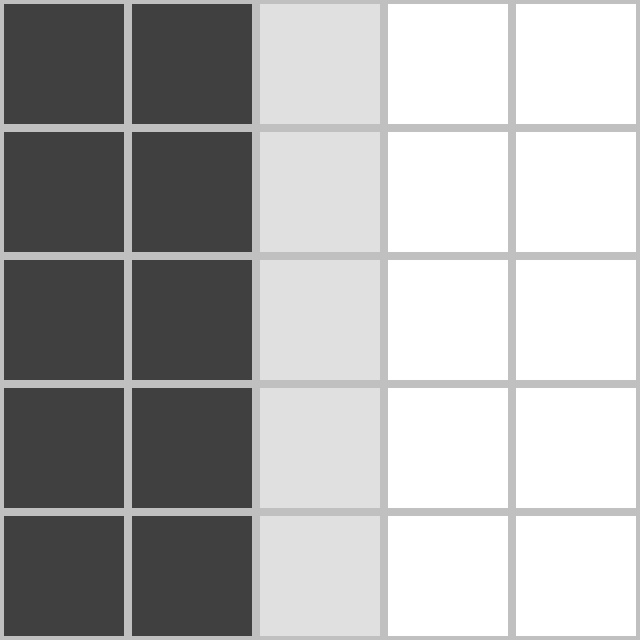
\includegraphics[width=5cm]{oscillators/phoenix_proof_1.png}};
			
			\letternode{2}{4}{A}
			\letternode{2}{3}{B}
			\letternode{2}{2}{C}
			\letternode{3}{4}{J}
			\letternode{3}{3}{K}
			\letternode{3}{2}{L}
			\letternode{4}{3}{X}
			\end{tikzpicture}}
		\caption{A diagram illustrating the fact that no phoenix can extend outside of its original bounding box (depicted by the dark grey cells) by more than one cell (depicted by the light grey cells). In particular, if the phoenix is initially confined to the dark grey cells, then cell~X can never be born.}\label{fig:phoenix_proof_1}
	\end{figure}
	
	Suppose for a contradiction that some cell at a distance of~2 from the original bounding box is eventually born, and let X be the first such cell, which is born for the first time in generation~$n$. Then cells~J, K, and L in Figure~\ref{fig:phoenix_proof_1} must each have been alive in generation~$n-1$, and since the pattern is a phoenix, they must each have been dead in generation~$n-2$. However, for cell~K to be born in generation~$n-1$, each of cells~A, B, and C must have been alive in generation~$n-2$, and thus must be dead in generation~$n-1$. We have thus shown that in generation~$n-1$, cell~K is alive and has exactly two live neighbors (J and L) and thus lives on to generation~$n$, so the pattern is not actually a phoenix.
	
	The fact that every phoenix eventually evolves into an oscillator follows immediately: there are $2^{wh}$ different patterns that fit inside a $w \times h$ box, so any pattern that stays confined to such a box forever must return to a previous phase (and thus oscillate) after no more than $2^{wh}$ generations.
\end{proof}

Before proceeding, we note that the technique used in the proof of Theorem~\ref{thm:phoenix_oscillate} is actually a very common one: to prove that a pattern with a certain property does not exist, consider what happens to the pattern at one of its far edges. We will use this same general method to prove another theorem about phoenices momentarily, and we will use it again in Section~\ref{sec:speed_limits} to find bounds on how fast spaceships can travel.

Now that we know that all phoenices evolve into oscillators, we are left with the question of what periods they can have. We already saw an example of a period~2 phoenix, but to date no one has found any phoenices with period~3 or higher. The following theorem\footnote{This theorem was also originally proved by Stephen Silver in January 2000.} shows that no phoenix of period~3 exists.

\begin{theorem}[No Phoenices with Period 3]\label{thm:phoenix_p3}
	In Conway's Game of Life, there does not exist a phoenix oscillator with period~3.
\end{theorem}

\begin{proof}
	Suppose there were a phoenix with period~3. Consider the uppermost row in the rotor of the phoenix, and let A be the leftmost cell in that row that is in the rotor, as in Figure~\ref{fig:phoenix_proof_2}. Without loss of generality, suppose that cell~A is alive in generation~3.
	
	\begin{figure}[!htb]
		\centering\gridbox{1.5pt}{\begin{tikzpicture}[scale=0.6, every node/.style={transform shape}]%
			\node[inner sep=0pt,anchor=south west] (glider_loop) at (0.5,0.5) {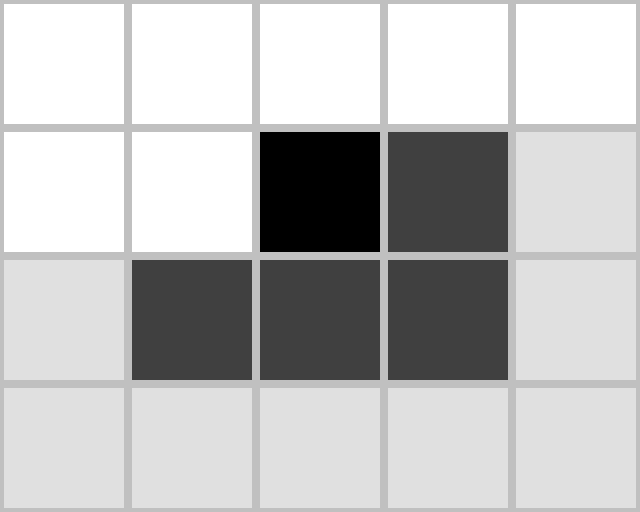
\includegraphics[width=5cm]{oscillators/phoenix_proof_2.png}};
			
			\letternode{3}{3}{A}
			\letternode{2}{2}{J}
			\letternode{3}{2}{K}
			\letternode{4}{3}{L}
			\letternode{4}{2}{M}
			\end{tikzpicture}}
		\caption{A diagram depicting the top-left corner of a hypothetical period~3 phoenix oscillator. Cell~A is the leftmost cell in the uppermost row of the oscillator, and exactly three of J, K, L, or M must be alive in the generation before A is alive.}\label{fig:phoenix_proof_2}
	\end{figure}
	
	We know that cell~A must have three neighbors that are alive in generation~2, and they must be three of the cells J, K, L, or M in Figure~\ref{fig:phoenix_proof_2}. Suppose (for a contradiction) that cell~K is alive in generation~2. Since K has at least two live neighbors in generation~2 (at least two of J, L, or M), it must in fact have at least four live neighbors (in order for it to die in generation~3). It follows that we can list K's (alive and dead) neighbors as follows:
	
	\begin{itemize}
		\item one cell (to its top-left) that is never alive,
		
		\item cell~A, which is alive in generation~3,
		
		\item at least four neighbors that are alive in generation~2, and
		
		\item exactly three neighbors (its parents) that are alive in generation~1.
	\end{itemize}
	
	Since none of the neighbors that are alive in generations~1, 2, or 3 can be the same (since it is a period~3 phoenix), we have shown that K has at least nine neighbors, which is a contradiction that shows that K must in fact be dead in generation~2. It follows that each of J, L, and M are alive in generation~2.
	\begin{figure}[!ht]
		\centering\gridbox{1.5pt}{\begin{tikzpicture}[scale=0.6, every node/.style={transform shape}]%
			\node[inner sep=0pt,anchor=south west] (glider_loop) at (0.5,0.5) {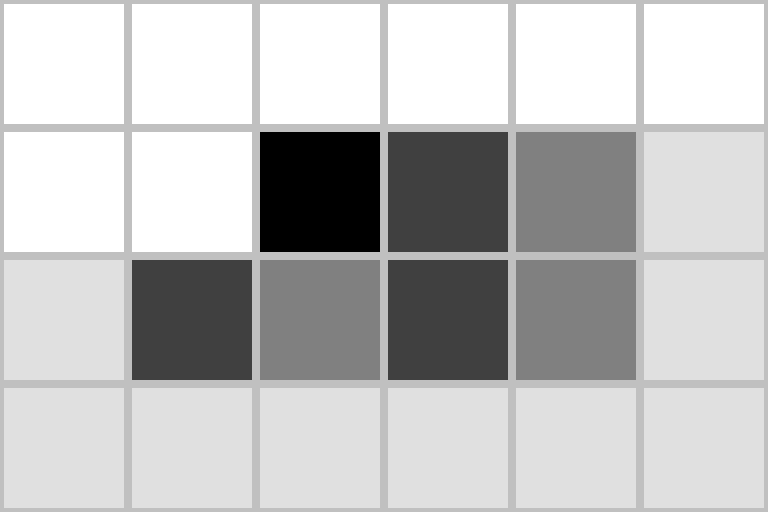
\includegraphics[width=6cm]{oscillators/phoenix_proof_3.png}};
			
			\letternode{3}{3}{A}
			\letternode{2}{2}{J}
			\letternode{3}{2}{K}
			\letternode{4}{3}{L}
			\letternode{4}{2}{M}
			\letternode{5}{3}{X}
			\letternode{5}{2}{Y}
			\end{tikzpicture}}
		\caption{A diagram that shows that no period~3 phoenix oscillator exists. Cell~A is alive in generation~3, cells J, L, and M are alive in generation~2, and cells K, X, and Y are alive in generation~1. Cell~X has only two neighbors (to its right and lower-right) that could potentially be alive in generation~0, so there was in fact no way for it to be born.}\label{fig:phoenix_proof_3}
	\end{figure}
	
	Since L must have three parents that are alive in generation~1, they must be cells K, X, and Y in Figure~\ref{fig:phoenix_proof_3}. However, there is then only room for cell~X to have at most two parents that are alive in generation~0 (in particular, the cell to its right and the cell to its lower-right), so it can't be born in generation~1, which is the contradiction that shows that this period~3 phoenix does not actually exist.
\end{proof}

A computer-assisted proof has also been used to show that no phoenices of period~5 exist,\footnote{This proof was completed by Alex Greason in September 2019.} but essentially nothing else is known about the (non-)existence of phoenices with period~4 or greater. On the other hand, if we relax the restriction on phoenices a bit and instead ask whether or not there exist higher-period oscillators with the property that every cell in the oscillator actually oscillates (i.e., the oscillator has no stator), it turns out that the answer is yes. For example, every cell in the period~3 oscillator displayed in Figure~\ref{fig:period_3_volatile} oscillates, even though it is not a phoenix.

\begin{figure}[!htb]
	\centering
	\patternimglink{0.1}{period_3_volatile}
	\caption{A period~3 oscillator with the property that every cell oscillates. It was found by Jason Summers in August 2012.}\label{fig:period_3_volatile}
\end{figure}


%%%%%%%%%%%%%%%%%%%%%%%%%%%%%%%%
\section{Notes and Historical Remarks}\label{sec:oscillators_notes}
%%%%%%%%%%%%%%%%%%%%%%%%%%%%%%%%

The search for new oscillators has been one of the most consistently active research areas throughout the history of Life. Much of its motivation comes from the omniperiodicity problem---it's remarkable that such a seemingly simple problem still remains unsolved after all these years, despite the various techniques that have been developed for constructing oscillators. To illustrate just how incomplete our methods of constructing and searching for oscillators are, consider the small period~$16$ oscillators displayed in Figures~\ref{fig:rich_p16} and~\ref{fig:rob_p16}. Despite their small size and simplicity, they were not discovered until July 2016 and February 2020, respectively, and they were found in possibly the least enlightening way possible---as a result of evolving computer-generated random soups (by apgsearch\index{apgsearch}).

\begin{figure}[!htb]
	\centering
	\begin{minipage}[b]{.48\textwidth}
		\centering
		\patternimglink{0.1}{rich_p16}
		\caption{\textbf{Rich's p16}\index{Rich's p16} is a period~16 oscillator that was found in a random soup by Rich Holmes in July 2016.}\label{fig:rich_p16}
	\end{minipage} \hfill %
	\begin{minipage}[b]{.48\textwidth}
		\centering
		\patternimglink{0.114201183432}{rob_p16}
		\caption{\textbf{Rob's p16}\index{Rob's p16} is a period~16 oscillator that was found in a random soup by Rob Liston in February 2020.}\label{fig:rob_p16}
	\end{minipage}
\end{figure}

However, oscillators also have great practical use, since sparkers in particular can be used for a great many purposes. We already saw that they can be used to create higher-period oscillators with composite periods, but they also form the basic building blocks of many of the large patterns that we will construct in later chapters. For example, the entirety of Chapter~\ref{chp:periodic_circuitry} is devoted to using oscillators to emulate logic circuits that can perform computation.

Many of the small billiard table oscillators that are known were found by David Buckingham, who discovered dozens of them throughout the 1970s and 1980s. Herschel tracks were also primarily his invention---he spent several years cataloguing patterns that moved B-heptominoes and Herschels from one place to another, and by October 1996 he had a complete toolkit capable of constructing oscillators and gliders guns with any period at least $61$.

Almost immediately, Paul Callahan used Herschel tracks to construct the first explicit stable glider reflector~\cite{BC98},\footnote{Although it had been known since the early 1970s that stable reflectors must exist in Life \cite{Wain74,BCG82}, no specific examples had been found prior to Callahan's construction.} which had a repeat time of $4{\thousep}840$ generations. It didn't take long for him to make some optimizations, resulting in a stable reflector with repeat time of 894 generations. Various optimizations were then made with the help of Dean Hickerson, getting the repeat time down to 747 in November 1996, followed by David Buckingham reducing the repeat time to 672 in May 1997, Stephen Silver reducing it to 623 in October 1997, Paul Callahan reducing it to 575 in November 1998, and finally Stephen Silver reducing it to 497 (as in the Silver reflector of Figure~\ref{fig:silver_reflector}) a few days later.

\begin{figure}[!htb]
	\centering\patternimglink{0.12}{period_56_herschel}
	\caption{A period~56 oscillator that was constructed using periodic Herschel conduits. It was built by Dietrich Leithner in December 1997.}\label{fig:period_56_herschel}
\end{figure}

A 180-degree stable reflector with repeat time of 202~generations, called the \textbf{boojum reflector},\footnote{In Lewis Carroll's epic poem \emph{The Hunting of the Snark}, a ``Boojum'' is a particularly dangerous type of Snark.} was found by Dave Greene in April 2001, and a 180-degree stable reflector with repeat time of 106~generations, called the \textbf{rectifier}\index{rectifier}, was found by Adam P. Goucher in March 2009 (see Exercise~\ref{exer:new_reflectors}). Finally, the Snark that we saw in Figure~\ref{fig:snark}, with a repeat time of just 43~generations, was found by Mike Playle in April 2013.

Although Buckingham's original Herschel conduits were used to construct oscillators with period~61 or higher, faster-recovering conduits can be used to create oscillators with period 58, 59, and 60 as well (see Exercise~\ref{exer:herschel_track_L112}). In December 1997, Dietrich Leithner found fast oscillating Herschel conduits that even allow for the construction of oscillators with period~56 and~57 (see Figure~\ref{fig:period_56_herschel} and Exercises~\ref{exer:period_57_herschel} and~\ref{exer:period_56_herschel}). In fact, these oscillating conduits were used to construct the first known period~57 oscillator. % http://www.radicaleye.com/lifepage/patterns/p57/p57.html

Herschel tracks remain one of the pinnacles of Life technology to this day, although they have evolved somewhat---many objects other than Herschels and B-heptominoes can be moved around tracks and converted into each other. We will return to this topic and investigate it more thoroughly in Chapter~\ref{chp:stationary_circuitry}.


\filbreak


%%%%%%%%%%%%%%%%%%%%%%%%%%%%%%%%%
\section*{Exercises \hfill \normalfont\textsf{\small solutions to starred exercises on \hyperlink{solutions_oscillators}{page \pageref{solutions_oscillators}}}}
\label{sec:oscillators_exercises}
\addcontentsline{toc}{section}{Exercises}
\vspace*{-0.4cm}\hrulefill\vspace*{-0.3cm}\footnotesize\begin{multicols}{2}\vspace*{-0.4cm}\raggedcolumns\interlinepenalty=10000
	\setlength{\parskip}{0pt}\ifdefined\FORPRINTING\colorlet{ocre}{black}\else%
\fi
	%%%%%%%%%%%%%%%%%%%%%%%%%%%%%%%%%
	
	\begin{problemstar}\label{exer:billiard_tables} \probdiff{2}
		For each of the following boxes, use induction coils to crowd the red cells and then find something that you can put in the green cells so as to make a billiard table oscillator.\vspace*{-0.25cm}
		
		\begin{multicols}{2}
			\begin{enumerate}
				\item[\bf\color{ocre}(a)] \raisebox{-\height+0.5em}{\patternimg{0.1}{exercise_billiard_table_3x3}}
				
				\item[\bf\color{ocre}(c)] \raisebox{-\height+0.5em}{\patternimg{0.1}{exercise_billiard_table_4x4}}
				
				\item[\bf\color{ocre}(b)] \raisebox{-\height+0.5em}{\patternimg{0.1}{exercise_billiard_table_skew}}
			\end{enumerate}
		\end{multicols}
	\end{problemstar}
	
	
	\mfilbreak
	
	
	\begin{problem}\label{exer:billiard_table_5x3} \probdiff{3}
		Consider the $5 \times 3$ box displayed below as a potential starting point for constructing a billiard table oscillator.
		
		\begin{center}
			\patternimglink{0.1}{billiard_table_5x3}
		\end{center}
		
		\begin{enumerate}[label=\bf\color{ocre}(\alph*)]
			\item Find a stable way to crowd the red cells, just like we used two blocks and two snakes to crowd the outside of a $4 \times 3$ box in Section~\ref{sec:billiard_tables}.
			
			\item Show that there is no way to fill in the green cells so as to make this pattern an oscillator (try writing a computer program to help you).
		\end{enumerate}
	\end{problem}
	
	
	\mfilbreak
	
	
	\begin{problem}\label{exer:eater_1_replace_eater_2_osc} \probdiff{2}
		Replace the eater~1s with eater~2s in the oscillators from the following figures, without destroying the oscillator or altering its period:\smallskip
		
		\begin{enumerate}[label=\bf\color{ocre}(\alph*)]
			\item Figure~\ref{fig:roteightor},
			
			\item Figure~\ref{fig:period_22},
			
			\item Figure~\ref{fig:worker_bee},
			
			\item Figure~\ref{fig:period_52}, and
			
			\item Figure~\ref{fig:honey_thieves} (you can only replace two of the eater~1s). 
		\end{enumerate}
	\end{problem}
	
	
	\mfilbreak
	
	
	\begin{problem}\label{exer:extend_snacker} \probdiff{1}
		The period~$9$ snacker\index{snacker} oscillator from Figure~\ref{fig:snacker} can be stabilized on one side in ways other than using two eater~1s. Use the method shown below to extend this oscillator to one that makes use of at least 5 interacting pentadecathlons.
		
		\begin{center}
			\patternimglink{0.1}{exercise_extend_snacker}
		\end{center}
	\end{problem}
	
	
	\mfilbreak
	
	
	\begin{problemstar}\label{exer:t_sparkers}\index{T-nosed p4}\index{T-nosed p6} \probdiff{2}
		Use the sparks from either the T-nosed~p$4$ or the T-nosed~p$6$ (displayed below) and another oscillator of your choice to create non-trivial oscillators with...
		
		\begin{center}
			\patternimglink{0.1}{t_nosed_p6}
		\end{center}
		
		\begin{enumerate}[label=\bf\color{ocre}(\alph*)]
			\item period~$12$,
			
			\item period~$20$, and
			
			\item period~$24$.
		\end{enumerate}
	\end{problemstar}
	
	
	\mfilbreak
	
	
	\begin{problem}\label{exer:pipsquirter_reflectors}
		One of the primary uses of pipsquirters\index{pipsquirter} is their ability to reflect a glider when a boat, block, and eater~1 are placed nearby as shown below.
		
		\begin{center}
			\patternimglink{0.1}{pipsquirter_reflector}
		\end{center}
		
		\noindent The reflector above has period~$6$. Use this same reaction to create a glider reflector with...\smallskip
		
		\begin{enumerate}[label=\bf\color{ocre}(\alph*)]
			\item \probdiff{2} period~$7$, and
			
			\item \probdiff{3} period~$8$.
		\end{enumerate}
	\end{problem}


	\mfilbreak
	
	
	\begin{problemstar}\label{exer:p32_pi_hassler_eaters} \probdiff{1}
		Show how the snakes can be replaced by eater~1s in the period~$32$ ``gourmet''\index{gourmet} oscillator from Figure~\ref{fig:p32_pi_hassler}.
	\end{problemstar}
	
	
	\mfilbreak
	
	
	\begin{problem}\label{exer:volcanoes}
		Several period~$4$ and~$5$ lightweight, middleweight, and heavyweight supervolcanoes\index{supervolcano}\index{lightweight!supervolcano}\index{middleweight!supervolcano}\index{heavyweight!supervolcano} are displayed below,\footnote{The p$4$ LW supervolcano was found by Noam Elkies in 2010, the p$5$ MW supervolcano was found by Dongook Lee in 2019, the p$5$ HW supervolcano was found by Karel Suhajda 2004, and the rest were found by Matthias Merzenich in 2010.} and they are particularly useful due to how far they push away their sparks.
		
		\begin{center}
			\patternimglink{0.07}{supervolcanoes}
		\end{center}
		
		\begin{enumerate}[label=\bf\color{ocre}(\alph*)]
			\item \probdiff{2} Use the sparks from two supervolcanoes to construct a period~$20$ oscillator.
			
			\item \probdiff{2} Use a supervolcano and a thumb sparker to create a non-trivial period~$20$ oscillator.
			
			\item \probdiff{3} Use a supervolcano to help you construct a T-tetromino shuttle.
		\end{enumerate}
	\end{problem}
	
	
	\mfilbreak
	
	
	\begin{problemstar}\label{exer:pi_hassle} \probdiff{4}
		A domino spark can be used to rotate a pi-heptomino\index{pi-heptomino} by 90 degrees in $8$~generations, as shown below. Use this reaction to create a period~$32$ oscillator. [Hint: The spark from a figure eight does not quite work. Try some other domino sparkers---you may need to weld them together in order to make them fit together closely enough.]
		\begin{center}
			\patternlink{exercise_pi_hassle}{\vcenteredhbox{\patternimg{0.1}{exercise_pi_hassle_0}} \vcenteredhbox{\genarrow{2}} \vcenteredhbox{\patternimg{0.1}{exercise_pi_hassle_2}} \vcenteredhbox{\genarrow{6}} \vcenteredhbox{\patternimg{0.1}{exercise_pi_hassle_8}}}
		\end{center}
	\end{problemstar}
	
	
	\mfilbreak
	
	
	\begin{problemstar}\label{exer:high_period_sparkers} \probdiff{2}
		This exercise introduces some sparkers with higher period than we saw in Section~\ref{sec:sparkers}. For each of them, determine their period, find an accessible spark that they emit (the spark might only be present in one of its phases not displayed below), and use that spark to construct a non-trivial oscillator with higher period.
		\begin{multicols}{2}
			\begin{enumerate}
				\item[\bf\color{ocre}(a)] \raisebox{-\height+0.5em}{\patternimglink{0.1}{exercise_high_period_sparker_13}}
				
				\item[\bf\color{ocre}(c)] \raisebox{-\height+0.5em}{\patternimglink{0.1}{exercise_high_period_sparker_32}}
				
				\item[\bf\color{ocre}(b)] \raisebox{-\height+0.5em}{\patternimglink{0.1}{exercise_high_period_sparker_31}}
			\end{enumerate}
		\end{multicols}
	\end{problemstar}
	
	
	\mfilbreak
	
	
	\begin{problem}\label{exer:b_heptomino_hassle} \probdiff{2}
		A dot spark and an eater~2 can be used to reflect a B-heptomino\index{B-heptomino} in $11$~generations, as shown below. Use this reaction to create a period~$22$ oscillator.
		\begin{center}
			\patternlink{b_heptomino_hassle}{\vcenteredhbox{\patternimg{0.1}{b_heptomino_hassle_0}} \vcenteredhbox{\genarrow{5}} \vcenteredhbox{\patternimg{0.1}{b_heptomino_hassle_5}} \vcenteredhbox{\genarrow{6}} \vcenteredhbox{\patternimg{0.1}{b_heptomino_hassle_11}}}
		\end{center}
	\end{problem}
	
	
	\mfilbreak
	
	
	\begin{problem}\label{exer:pond_block_hasslers} \probdiff{3}
		Use the hassling reaction from Figure~\ref{fig:p27_hassler} to create an oscillator with...\smallskip
		
		\begin{enumerate}[label=\bf\color{ocre}(\alph*)]
			\item period~$24$, and% blocker works
			
			\item period~$21$, using the following p$7$ duoplet sparker:
			
			\begin{center}
				\patternimglink{0.1}{p7_duoplet_sparker}
			\end{center}
		\end{enumerate}
	\end{problem}
	
	
	\mfilbreak
	
	
	\begin{problemstar}\label{exer:p44_pi_hassler} \probdiff{3}
		A partial pi-heptomino hassler is displayed below. Complete it by placing sparkers so that domino sparks are present at the indicated locations $33$~generations after the phase shown here.
		
		\begin{center}
			\patternimglink{0.1}{exercise_pi_heptomino_hassler}
		\end{center}
		
		\noindent [Hint: What will the period of this oscillator be? Make sure that the hassler you pick has a compatible period.]
	\end{problemstar}
	
	
	\mfilbreak
	
	
	\begin{problem}\label{exer:pentadecathlon_relay_180} \probdiff{2}
		Use two pentadecathlons to construct a glider loop oscillator with period 180.
	\end{problem}
	
	
	\mfilbreak
	
	
	\begin{problem}\label{exer:snark_relay_180} \probdiff{2}
		Use four Snarks to construct an oscillator with period 180.
	\end{problem}
	
	
	\mfilbreak
	
	
	\begin{problemstar}\label{exer:six_snark_relay} \probdiff{2}
		Create a glider loop (of any period) that makes use of exactly six Snarks.
	\end{problemstar}
	
	
	\mfilbreak
	
	
	\begin{problemstar}\label{exer:snark_weld} \probdiff{3}
		Sometimes it is useful to weld together reflectors, just like we welded together eaters in the previous chapter.\smallskip
		
		\begin{enumerate}[label=\bf\color{ocre}(\alph*)]
			\item Weld together the following two partial Snarks (modify only the light gray cells), thus creating a single still life that can reflect gliders from two different sides.
			\begin{center}
				\patternimglink{0.1}{exercise_fused_snarks}
			\end{center}
			
			\item Modify the reflector from part~(a) to create a single reflector that can reflect gliders coming from four different sides.
		\end{enumerate}
	\end{problemstar}
	
	
	\mfilbreak
	
	
	\begin{problemstar}\label{exer:snark_creates_honeyfarm} \probdiff{2}
		The Snark\index{Snark} reflector works by converting the input glider into another object that we have seen before, and then converting that object into the output glider. What is the name of the intermediate object?
	\end{problemstar}
	
	
	\mfilbreak
	
	
	\begin{problemstar}\label{exer:almost_snark} \probdiff{2}
		The pattern displayed below\footnote{Found by Tanner Jacobi in 2015.} might be called an ``almost Snark'', since it can \emph{almost} be used as a $90$-degree glider reflector. Describe what goes wrong and why it cannot reflect more than one glider.
		
		\begin{center}
			\patternimglink{0.1}{almost_snark}
		\end{center}
	\end{problemstar}
	
	
	\mfilbreak
	
	
	\begin{problem}\label{exer:buckaroo_loop} \probdiff{3}
		Create a glider loop that uses at least one buckaroo and at least one twin bees shuttle. What is the smallest possible period of such an oscillator? %SOLUTION: lcm(30,46) = 690
	\end{problem}
	
	
	\mfilbreak
	
	
	\begin{problem}\label{exer:new_reflectors} \probdiff{3}
		For each of the following 180-degree stable reflectors, construct an oscillator that works by using two copies of the reflector to bounce a glider back and forth, and determine what the possible periods of such oscillators are.\smallskip
		
		\begin{enumerate}[label=\bf\color{ocre}(\alph*)]
			\item \textbf{Boojum reflector}:\index{boojum reflector} \\ \raisebox{-\height+0.5em}{\patternimg{0.1}{boojum_reflector}}\\[0.5em]
			
			\item \textbf{Rectifier}:\index{rectifier} \\ \raisebox{-\height+0.5em}{\patternimg{0.1}{rectifier}}
		\end{enumerate}
	\end{problem}
	
	
	\mfilbreak
	
	
	\begin{problem}\label{exer:machine_gun} \probdiff{3}
		Recall the 64-generation 90-degree Herschel conduit in Figure~\ref{fig:herschel_64}.\smallskip
		
		\begin{enumerate}[label=\bf\color{ocre}(\alph*)]
			\item Use four copies of the conduit to create a gun that shoots 4 gliders every 256 generations.
			
			\item Modify the pattern from part~(a) to create a period 256 oscillator. % just add eaters on the outside
			
			\item Can you add additional Herschels to this track to make an oscillator with period~128 or~64? Either explicitly construct an example or explain the problem that arises. % No, can't do this: the gliders that the Herschels emit interfere with the previous Herschels on the track.
		\end{enumerate}
	\end{problem}
	
	
	\mfilbreak
	
	
	\begin{problemstar}\label{exer:traffic_jam} \probdiff{4}
		Two reactions that move traffic lights and T-tetrominoes are displayed below (the top one is called a \textbf{traffic jam}\index{traffic jam}):
		
		\noindent\begin{center}
			\patternlink{traffic_jam}{\vcenteredhbox{\patternimg{0.1}{traffic_jam_0}} \vcenteredhbox{\genarrow{25}} \vcenteredhbox{\patternimg{0.1}{traffic_jam_25}}}
		\end{center}\vspace*{-0.35cm}
		
		\noindent\begin{center}
			\patternlink{t_tetromino_hassle_3}{\vcenteredhbox{\patternimg{0.1}{t_tetromino_hassle_3_0}} \vcenteredhbox{\genarrow{3}} \vcenteredhbox{\patternimg{0.1}{t_tetromino_hassle_3_3}} \vcenteredhbox{\genarrow{4}} \vcenteredhbox{\patternimg{0.1}{t_tetromino_hassle_3_7}} \vcenteredhbox{\genarrow{4}} \vcenteredhbox{\patternimg{0.1}{t_tetromino_hassle_3_11}}}
		\end{center}
		
		\noindent Use these reactions (and optionally any of the other T-tetromino hassling reactions we have seen) to create an oscillator.
	\end{problemstar}
	
	
	\mfilbreak
	
	
	\begin{problemstar}\label{exer:traffic_jam_reflect} \probdiff{3}
		What type of sparks does the traffic jam reaction from the top of Exercise~\ref{exer:traffic_jam} produce? Use this spark and the oscillator constructed in Exercise~\ref{exer:traffic_jam} to create a periodic glider reflector.
	\end{problemstar}
	
	
	\mfilbreak
	
	
	\begin{problem}\label{exer:herschel_track_1} \probdiff{3}
		Use the R64 and Fx77 conduits to construct Herschel track oscillators or guns with the following periods.
		
		\noindent [Hint: Mimic our construction in Figure~\ref{fig:herschel_track_oscillators}.]\smallskip
		
		\begin{enumerate}[label=\bf\color{ocre}(\alph*)]
			\item Period~$218$ oscillator.
			
			\item Period~$62$ oscillator.
			
			\item Period~$62$ glider gun.
			
			\item Period~$61$ oscillator.
			
			\item Period~$63$ glider gun.
		\end{enumerate}
	\end{problem}
	
	
	\mfilbreak
	
	
	\begin{problem}\label{exer:herschel_track_2_what_periods} \probdiff{2}
		By placing different numbers of Herschels on the track from Figure~\ref{fig:herschel_track_2}, oscillators of which periods can be created?
	\end{problem}
	
	
	\mfilbreak
	
	
	\begin{problem}\label{exer:herschel_track_L112}
		Consider the Herschel conduit displayed below, which rotates a Herschel counter-clockwise in 112 generations and has a repeat time of 58 generations. This conduit is called \textbf{L112}\index{L112}.
		
		\begin{center}
			\patternimglink{0.1}{L112}
		\end{center}
		
		\begin{enumerate}[label=\bf\color{ocre}(\alph*)]
			\item \probdiff{3} Construct a period~109 oscillator by using only the L112 and Fx77 conduits (and possibly some eaters to destroy stray gliders).
			
			\item \probdiff{4} The L112 conduit has a slightly faster repeat time than the R64 conduit (58 generations instead of 61). Use the L112 and Fx77 conduits to create an oscillator with period~58, 59, or 60.
		\end{enumerate}
	\end{problem}


	\mfilbreak
	
	
	\begin{problemstar}\label{exer:phoenix_bb} \probdiff{3}
		Based on the phoenix oscillator shown in Figure~\ref{fig:phoenix}, we might be tempted to guess that Theorem~\ref{thm:phoenix_oscillate} can be improved to show that no phoenix can ever leave its original bounding box at all. Show that this conjecture is false. That is, find a phoenix that does in fact leave its original bounding box.
	\end{problemstar}
	
	
	\mfilbreak
	
	
	\begin{problem}\label{exer:period_57_herschel} \probdiff{4}
		Consider the (oscillating!) Herschel conduit displayed below, which rotates a Herschel counter-clockwise and flips it in 65 generations, and has a repeat time of 57 generations. Construct a period~57 oscillator by using this new conduit and the Fx77 conduit (and possibly some eaters to destroy stray gliders).
		\begin{center}
			\patternimglink{0.1}{period_57_herschel}
		\end{center}
	\end{problem}
	
	
	\mfilbreak
	
	
	\begin{problem}\label{exer:period_56_herschel} \probdiff{3}
		Consider the period~56 Herschel track oscillator depicted in Figure~\ref{fig:period_56_herschel}. Break this oscillator down into its individual conduits, and for each conduit state (a) how many generations it takes a Herschel to traverse the conduit, and (b) what the conduit's repeat time is. Also break down each conduit into still lifes, oscillators, and eaters that we have seen earlier.
	\end{problem}
	
	
	\mfilbreak
	
	
	\begin{problemstar}\label{exer:p4_oscillator} \probdiff{4}
		Prove that there is no period~4 oscillator with exactly one cell that oscillates at the full period.
	\end{problemstar}


	\mfilbreak
	
	
	\begin{problem}\label{exer:p4_oscillator_impb} \probdiff{4}
		Prove that there is no period~4 oscillator whose rotor consists of exactly $4$ cells, which take turns being alive for one generation out of each four.
	\end{problem}
% SOLUTION (from Dean Hickerson): If you mean that there are only 4 active cells, A, B, C, and D, such that exactly one is alive in each phase, then there's no such object. For suppose that A is alive in gen 0 and B is alive in gen 1. Then B must be born in gen 1, so it has either 2 or 3 neighbors among the stable cells (2 if B is adjacent to A, 3 otherwise). But then B must survive into gen 2, a contradiction.
	
	
	\mfilbreak
	
	
	\begin{problemstar}\label{exer:period_3_volatile} \probdiff{2}
		The period~3 oscillator presented in Figure~\ref{fig:period_3_volatile} was constructed by putting together the various period~3 ``pieces'' displayed below. Use these same pieces to construct a larger period~3 oscillator with at least 200 live cells in one of its phases.
		\begin{center}
			\patternimglink{0.085}{period_3_volatile_pieces}
		\end{center}
	\end{problemstar}
	
	%% EXERCISE END COMMANDS
\end{multicols}
\normalsize\vspace*{0.01cm}\ifdefined\FORPRINTING\colorlet{ocre}{rawocre}\else%
\fi
%% DONE EXERCISE END COMMANDS
